\documentclass[12pt,UTF8]{ctexbook}
\usepackage{ctex}
\usepackage{array}
\usepackage{graphicx}
\usepackage{wrapfig}
\usepackage[table,dvipsnames]{xcolor}
\usepackage{tabularx}
\usepackage{amsmath}
\usepackage{amssymb}
\usepackage{xfrac}
\usepackage{eucal}
\usepackage{titlesec}
\usepackage{amsthm}
\usepackage{tikz-cd}
\usepackage{enumitem}
\usepackage{verbatim}
\usepackage{fontspec,xunicode,xltxtra}
\usepackage{xeCJK} 
\usepackage{caption}

\definecolor{gl}{RGB}{246, 252, 240}
\definecolor{gd}{RGB}{236, 244, 230}
\definecolor{bg}{RGB}{242, 244, 228}


\setCJKmainfont[BoldFont=STZhongsong]{STSong}
\setCJKmonofont{simkai.ttf} % for \texttt
\setCJKsansfont{simfang.ttf} % for \textsf
\setlength\parskip{8pt}
\setlength{\fboxsep}{12pt}
\renewcommand\thesection{\arabic{chapter}.\arabic{section}}
\newcommand{\arccot}{\operatorname{arccot}}
\newtheorem{df}{定义}[section] 
\newtheorem{pp}{命题}[section]
\newtheorem{tm}{定理}[section]
\newtheorem{ex}{例子}[section]
\newtheorem{et}{例题}[section]
\newtheorem{sk}{思考}[section]
\newtheorem*{po}{公理}
\newtheorem*{so}{解答}
\newenvironment{proof2}{\paragraph{\textbf{证明:}}}{\hfill$\square$}
\newtheorem{xt}{习题}[section]
\newtheorem{cor}{推论}[pp]
% 列举环境的行间距
\setenumerate[1]{itemsep=0pt,partopsep=0pt,parsep=0pt,topsep=0pt}
\setitemize[1]{itemsep=0pt,partopsep=0pt,parsep=0pt,topsep=0pt}
\setdescription{itemsep=0pt,partopsep=0pt,parsep=0pt,topsep=0pt}
% 章节字体大小
\titleformat{\section}{\zihao{-2}\bfseries}{ \thesection }{16pt}{}
% 封面
\title{\zihao{0} \bfseries 第一册}
\author{\zihao{2} \texttt{大青花鱼}}
% \date{\bfseries\today}
\date{}
% 正文
\begin{document}
\maketitle
\tableofcontents
\newpage

\chapter{数列初步}

\section{数列的基本概念}

\begin{ex}
    \mbox{}\\
    \indent 1. 把自然数的倒数排成一列:
$$ 1,\,\,\, \frac{1}{2}, \,\,\, \frac{1}{3}, \,\,\,\frac{1}{4}, \,\,\,\frac{1}{5}, \cdots $$

2. 把圆周率按个位,十分位、百分位、千分位等等截断,得到一列数:
$$  3,\,\,\, 3.1,\,\,\, 3.14,\,\,\, 3.141,\,\,\, 3.1415, \cdots   $$

    3. 把班上同学的身高(厘米)按学号排列:
$$ 165,\,\,\, 173,\,\,\, 169,\,\,\, 178, \,\,\,171.5,\,\,\, 176, \cdots  $$
\end{ex}
把数按照一定顺序排列起来,叫做\textbf{数列}。数列中的每一个数叫做数列的一\textbf{项}。
按照顺序,各项分别称为数列的第$1$项、第$2$项,等等。
比如,例$1$中的数列第$2$项是$\frac{1}{2}$,例$2$中的数列第$3$项是$3.14$。

数列的项和序数有一一对应的关系,这告诉我们,数列的本质是正整数集或其子集$[1\ldots N]$到数域的函数。
定义域是$[1\ldots N]$的数列,项数有限,称为\textbf{有穷数列};定义域是正整数集的数列,项数无限,叫做\textbf{无穷数列}。
我们一般把数列记作:
$$ a_1, a_2, \cdots, a_n, \cdots $$
其中$a_n$是数列的第$n$项。项数$n$也叫做\textbf{下标}。
为了方便,我们在行文中会把以上数列记作$\{a_n\}_{n\in\mathbb{Z}^+}$(无穷数列)
或$\{a_n\}_{n\in[1\ldots N]}$(有穷数列),或简单记作$\{a_n\}$。
比如,例$1$中的数列可以记为$\left\{\frac{1}{n}\right\}_{n\in\mathbb{Z}^+}$。
作为函数,如果某数列的序数和项之间的对应关系可以用一个公式来表示,
我们就把这个公式称为该数列的\textbf{通项公式}。比如,例$1$中的数列,通项公式是$a_n = \frac{1}{n}$;
而例$3$中的数列,我们不知道通项公式。有通项公式的数列,只要把序数代入公式,就能得到该项的值。
比如,例$1$中的数列,第$100$项是$\frac{1}{100}$。

我们把各项不断增大(减小)的数列称为\textbf{单调递增(递减)数列}。“单调”一词,表示数列各项增减方向保持一致。
换句话说,如果数列$\{a_n\}_{n\in\mathbb{Z}^+}$从第一项起,总有$a_{n+1} \geqslant a_n$,
就说它是\textbf{单调递增数列};如果总有$a_{n+1} \leqslant a_n$,就说它是\textbf{单调递减数列}。如果要求不能有相等的项,
就称为\textbf{严格单调递增(递减)数列}。

研究数列的一个基本目的,是对数列进行求和。比如,一垛炮弹有$8$层,顶层有$1$个炮弹,第$2$层有$4$个,
第$3$层有$9$个,……,第$8$层有$64$个,我们希望知道一共有几个炮弹。把各层炮弹个数记为数列:$a_1 = 1$
$$ a_1 = 1, a_2 = 4, \cdots, a_8 = 64 $$
我们把数列的和记为$S_8 = a_1 + a_2 + \cdots + a_8$。为了方便,我们也用\textbf{求和符号}$\sum$表示数列的和:$S_8 = \sum_{i=1}^8 a_i$。

对于无穷数列,我们还无法定义数列的和,只能定义它的\textbf{部分和}:$S_N = \sum_{i=1}^N a_i$。我们把$S_N$称为数列$\{a_n\}$的前$N$项和。比如,例$1$中的数列的前$4$项和为:
$$ S_4 = 1 + \frac{1}{2} + \frac{1}{3} + \frac{1}{4} =  \frac{25}{12}. $$

\begin{sk}
    \mbox{}\\
    \indent 1. 小明把正整数倒数组成的数列记为
    $$a_1 = 1, a_2 = \frac12, \cdots, a_n = \frac1n, \cdots$$
    \indent 小红把正整数倒数组成的数列记为
    $$a_0 = 1, a_1 = \frac12, \cdots, a_n = \frac{1}{n+1}, \cdots$$
    \indent 这两种记法有什么不同?\\
    \indent 2. 一般来说,用自然数作序数的数列$\{a_n\}_{n\in\mathbb{N}}$和用正整数作序数的数列$\{a_n\}_{n\in\mathbb{Z}^+}$有什么关系?有什么差别?
    使用整数作序数的数列$\{a_n\}_{n\in\mathbb{Z}}$呢?\\
    \indent 3. 是否能用有理数做数列的序数?实数呢?    
\end{sk}

\begin{xt}
    \mbox{}\\
\indent 1. 根据以下数列的通项公式,写出数列的前$5$项:\\
\indent 1.1. $a_n = n^2$ \\
\indent 1.2. $a_n = (-1)^n \cdot n$ \\
\indent 1.3. $a_n = \frac{n}{n+3}$ \\
\indent 1.4. $a_n = 2^n - 1$ \\
\indent 1.5. $a_n = \frac{(-2)^n + n - 1}{n^2 + 1}$ \\
\indent 2.根据以下数列的通项公式,计算数列的前$5$项和与前$7$项和: \\
\indent 2.1. $a_n = n^2$ \\
\indent 2.2. $a_n = (-1)^{n+1} \cdot n$ \\
\indent 2.3. $a_n = \frac{2}{n(n+1)}$ \\
\indent 2.4. $a_n = 2^n$ \\
\indent 2.5. $a_n = (n+1)2^{n}$ \\
\indent 3. 已知数列$\{a_n\}_{n\in\mathbb{Z}^+}$,如何构造一个数列$\{b_n\}_{n\in\mathbb{Z}^+}$,
使得它的前$n$项和是$a_n$?
\end{xt}

无穷数列之间(或项数相同的有穷数列之间),作为函数,可以进行函数之间的四则运算。
比如,设无穷数列$\{a_n\}$和$\{b_n\}$的通项公式分别是$a_n = n - 1$、$b_n = 2n$,
那么对任意正整数$n$,$a_n + b_n = 3n - 1$。
我们定义通项公式为$c_n = 3n - 1$的数列$\{c_n\}$为$\{a_n\}$与$\{b_n\}$的和,也就是说,
我们定义数列的加法:$\{a_n\} + \{b_n\} = \{a_n + b_n\}$。

可以验证,数列的加法满足交换律和结合律。我们称每项都等于同一个数的数列为\textbf{常数列},
任何数列加上常数列$\{0\}$都等于自己。

同理,我们可以定义数列的减法和乘法。它们满足的运算律和有理数的运算律一致。
任何数列乘以$\{1\}$都得到自己。如果我们把所有取值为实数的数列的集合记为$\mathbb{R}^\mathbb{N}$,
那么$\mathbb{R}^\mathbb{N}$和$\mathbb{Z}$一样,可以“装载”加法、减法和乘法。
其中的常数列$\{0\}$、$\{1\}$就相当于整数$0$和$1$。

此外,给定数列$\{a_n\}$和实数$t$,我们可以把$\{a_n\}$的每一项乘以$t$得到一个新数列:
$t\cdot \{a_n\} = \{t\cdot a_n\}$,这个运算称为\textbf{数乘运算}。数乘运算和数、数列的四则运算相容。
\begin{align}
    \forall  \,\, s, t \in \mathbb{R}, \,\,\, \forall \,\, \{a_n\}, \,\,\,& s \cdot (t\cdot \{a_n\}) = (s\cdot t)\cdot \{a_n\}, \notag \\
    & (s + t) \cdot \{a_n\} = (s\cdot \{a_n\}) + (t\cdot \{a_n\}). \notag \\
    \forall  \,\, t \in \mathbb{R}, \,\,\, \forall \,\, \{a_n\}, \,\, \{b_n\},\,\,\, & t \cdot (\{a_n\} + \{b_n\}) = (t \cdot \{a_n\}) + (t \cdot \{b_n\}). \notag 
\end{align}

无穷数列还可以进行函数操作。比如,我们定义函数$f:\,\,x\mapsto x^2 - 3$,
数列$\{a_n\}$的每一项经过$f$映射到$f(a_n) = f(n-1) = (n-1)^2 - 3 = n^2 - 2n - 2$。
那么数列$\{n^2-2n-2\}$就可以称为$\{a_n\}$经过$f$的\textbf{像数列}。
换句话说,我们用实值函数$f$定义了一个$\mathbb{R}^\mathbb{N}$到$\mathbb{R}^\mathbb{N}$的映射。

另一种对数列的操作方法是通过下标。设$g$是从正整数集映射到正整数集的函数,
比如$g:\,\, n \mapsto 3n - 2$。从$\{a_n\}$出发,考虑数列$\{u_n\}$:$u_n = a_{g(n)} = a_{3n-2}$。
这样定义的$\{u_n\}$称为用$g$从$\{a_n\}$中提取的数列。要注意的是,$g$不一定把$\{a_n\}$中每项恰好提取一次,比如
$$ a_1, a_1, a_2, a_2, a_3, a_3, a_4, a_4, \cdots $$
这样的数列也是从$\{a_n\}$中提取的。如果对任何正整数$n$,函数$g$满足$g(n+1) > g(n)$,
用$g$从$\{a_n\}$中提取的数列就可以看作是从前到后挑出一部分项得到的。这样的数列称为$\{a_n\}$的\textbf{子列}。

\begin{sk}
    \mbox{}\\
\indent 1. 给定数列$\{a_n\}$,它的前$n$项和可以构成一个数列$\{S_n\}$,如何用$\{S_n\}$中的项表示$a_n$?
记$v_n$为$\{a_n\}$前$n$项乘积,能否用数列$\{v_n\}$中的项表示$a_n$?\\
\indent 2. 记平面向量的集合为$\mathbb{V}$,
所有从$\mathbb{R}^\mathbb{N}$到$\mathbb{R}^\mathbb{N}$的映射的集合为$\mathfrak{F}(\mathbb{R}^\mathbb{N})$。
$\mathfrak{F}(\mathbb{R}^\mathbb{N})$和$\mathbb{V}$、$\mathbb{Z}$有什么共同点?有什么不同点?\\
\indent 3. 记所有从正整数集到正整数集的函数的集合为$\mathfrak{F}(\mathbb{Z}^+)$,
数列$\{a_n\}$经过$\mathfrak{F}(\mathbb{Z}^+)$中某个函数$g$可以提取出数列$\{b_n\}$。
$g$满足什么条件时,可以找到另一个$\mathfrak{F}(\mathbb{Z}^+)$中的函数$h$,
用$h$可以从$\{b_n\}$中提取出$\{a_n\}$?
\end{sk}

\begin{xt}
    \mbox{}\\
    \indent 1. 计算:$\{6n-1\} - \{3k^2 - k + 2\} \cdot \{2^m+1\}$ 。\\
    \indent 2. 已知定义在全体实数上的函数$f:\,\, x\mapsto 2x^2 - x - 4$,
    数列$\{a_n\}$的通项公式为$a_n = n + \frac{1}{n}$,计算$\{f(a_n)\}$。\\
    \indent 3. 另有定义在全体实数上的函数$g:\,\, x\mapsto 1 - \frac{1}{x}$,计算$\{(f - g)(a_n)\}$。
\end{xt}

研究实际问题的时候,我们可能不会直接得到数列的通项公式,而是各项之间的关系。来看以下的例子:
\begin{et}
培养一种乳酸菌,初始从$3$个单位起培养。每过一定时间,等乳酸菌数量翻倍后,
取出$1$个单位的样本做化验观察,其余继续培养。问每次取出化验后,乳酸菌的数量是几个单位?
\end{et}
\begin{so}
设初始数量为$a_0$,第$n$次取出化验后乳酸菌数量为$a_n$个单位。则数列$\{a_n\}$中的项满足以下的关系:
$$ \forall n \in \mathbb{N}, \quad a_{n+1} = 2a_n - 1. $$
\end{so}
这样的关系称为数列的\textbf{递推关系},相关公式称为\textbf{递推公式}。
以上公式中,已知$a_0$的值,就能推出$a_1$,继而次第推出$a_2$、$a_3$,等等。
$a_0 = 3$,所以$a_1 = 2\cdot 3 - 1= 5$,$a_2 = 2\cdot 5 - 1= 9$,$a_3 = 2\cdot 9 - 1= 17$……

根据递推关系,已知$a_1$,想要算出$a_{100}$,就必须依次算出$a_2,a_3,\cdots,a_{99}$。
很多时候,我们希望从各项之间的关系,推出通项公式,以更方便地了解数列的性质。

如何从递推关系得出通项公式呢?并没有简便的统一方法。
常见的做法是将递推关系转化为一些已知通项公式的数列的递推关系,再反推出原数列的通项公式。
下面我们会详细介绍。

\begin{xt}
\mbox{}\\
已知数列的递推公式如下,求数列的前$7$项:\\
\indent 1. $a_1 = 1$,$\forall n \geqslant 1, \,\,\, a_{n+1} = 1 - 2a_n.$\\
\indent 2. $a_1 = 1$,$\forall n \geqslant 1, \,\,\, a_{n+1} = 1 + \frac{1}{a_n - 1}.$\\
\indent 3. $a_1 = 1, \,\, \, a_2 = 3$,$\forall n \geqslant 1, \,\,\, a_{n+2} = 4 + a_n - a_n^2.$\\
\indent 4. $a_1 = 1, \,\, \, a_2 = 1$,$\forall n \geqslant 1, \,\,\, a_{n+2} = a_n +a_{n+1}.$\\
\indent 5. $a_1 = 1, \,\, \, a_2 = 3$,$\forall n \geqslant 1, \,\,\, a_{n+2} = a_n(4 - a_{n+1}).$
\end{xt}

\section{等差数列}
来看这样一个数列:
$$ 1,\,\,3,\,\,5,\,\,7,\,\,9,\,\,11,\,\, 13. $$
这个数列有一个特点:从第二项起,每一项减去前一项的差总是$2$。

一般地,如果某个数列从第二项起,每一项减去前一项的差是同一个常数,
就说这个数列是\textbf{等差数列}。这个常数叫做等差数列的\textbf{公差},通常用字母$d$表示。
比如,数列$2,5,8,11,14$的公差是$3$,$19,15,11,7,3,-1$的公差是$-4$。

如果数列$\{a_n\}$的公差是$d$,那么:
\begin{align}
a_2 &= a_1 + d \notag \\
a_3 &= a_2 + d = a_1 + 2d \notag \\
a_4 &= a_3 + d = a_1 + 3d \notag \\
&\quad \vdots \notag \\
a_n &= a_1 + (n-1)d \notag 
\end{align}
等差数列的通项公式是:
$$a_n = a_1 + (n-1)d.$$
\begin{et}
已知无穷等差数列$1,\,\,8,\,\,15, \cdots$,求它的第$30$项。
\end{et}
\begin{so}
等差数列第一项是$1$,公差是$8-1=7$,所以通项公式是$a_n = 1 + (n-1)\cdot 7 = 7n - 6$。第$30$项$a_{30} = 7\cdot 30 - 6 = 204$。
\end{so}
\begin{et}
已知$\{a_n\}_{n\in\mathbb{N}}$是等差数列,$a_1 = 4$, $a_3 = 9$ ,问$94$是否在数列中?如果是的话,是第几项?
\end{et}
\begin{so}
设公差为$d$,则$a_3 = a_1 + 2d$。代入$a_1$、$a_3$的值,解得$d = 2.5$。于是通项公式为$a_n = 4 + (n-1)\cdot 2.5 = 2.5n + 1.5$。如果有$a_n = 94$,即$2.5n + 1.5=94$,解得$n = 37$。因此$94$在数列中,是第$37$项。
\end{so}

设等差数列$\{a_n\}$的前$n$项和为$S_n$。能否方便地表示$S_n$呢?我们可以这样思考:
\begin{align}
a_{1} + a_{n} &= a_1 + a_1 + (n-1)d = 2a_1 + (n-1)d \notag \\
a_{2} + a_{n-1} &= a_1 + d + a_n - d = a_1 + a_n = 2a_1 + (n-1)d \notag \\
&\vdots \notag \\
a_{n-1} + a_{2} &= a_1 + (n-2)d + a_n - (n-2)d = a_1 + a_n =  2a_1 + (n-1)d \notag \\
a_{n} + a_{1} &= a_1 + a_n = 2a_1 + (n-1)d \notag 
\end{align}
把以上$n$个等式分边相加,就得到:
$$ S_n + S_n = n(a_1 + a_n) = 2na_1 + n(n-1)d. $$
也就是说,前$n$项和$S_n$可以写成
$$ S_n = \frac{n(a_1 + a_n)}{2} = na_1 + \frac{n(n-1)}{2}d. $$
这样我们可以方便地计算等差数列的前$n$项和。比如,求前$n$个自然数的和:$a_n = n-1 = 0 + (n-1)\cdot 1$,
$S_n = 0 + \frac{n(n-1)}{2}\cdot 1 = \frac{n(n-1)}{2}$。

\begin{xt}
    \mbox{} \\
    \indent 1. 在$8$和$36$之间插入$6$个数,使得这$8$个数成等差数列。\\
    \indent 2. 设数列$\{a_n\}_{n\in\mathbb{Z}^+}$为等差数列,证明$a_{n+2} + a_n = 2a_{n+1}$。\\
    \indent 3. 等差数列$\{a_n\}_{n\in\mathbb{Z}^+}$中,$a_1 = 0.3$,$a_n = 85.5$,$d = 0.6$,求$n$和$S_n$。\\
    \indent 4. 求前$n$个奇数$1,3,5,\cdots, 2n-1$的和。\\
    \indent 5. 直角三角形的三边成等差数列,求三边比例。\\
    \indent 6. 等差数列$\{a_n\}_{n\in\mathbb{Z}^+}$满足$a_1 = 1$,$a_{10}=43.3$,求$S_{20}$ 。    
\end{xt}

\section{等比数列}

来看这样一个数列:
$$ 1,\,\,2,\,\,4,\,\,8,\,\,16,\,\,32,\,\,64. $$
这个数列有一个特点:从第二项起,每一项除以前一项的商总是$2$。

一般地,如果某个数列从第二项起,每一项与前一项的比值是同一个常数,
就说这个数列是\textbf{等比数列}。这个常数叫做等比数列的\textbf{公比},通常用字母$q$表示。
比如,数列$2,6,18,54,162$的公比是$3$,$192,-48,12,-3,0.75$的公比是$-0.25$。

如果数列$\{a_n\}$的公比是$q$,那么:
\begin{align}
a_2 &= a_1 q  \notag \\
a_3 &= a_2 q = a_1 q^2 \notag \\
a_4 &= a_3 q = a_1 q^3 \notag \\
&\quad \vdots \notag \\
a_n &= a_1 q^{n-1} \notag 
\end{align}
等比数列的通项公式是:$a_n = a_1 q^{n-1}$。
\begin{et}
    已知无穷等比数列$1.2, \,\,1.8,\,\,2.7, \cdots$,求它的第$30$项。    
\end{et}
\begin{so}
等比数列第一项是$1$,公比是$1.8\div1.2=1.5$,所以通项公式是
$$a_n = 1.2 \cdot 1.5^{n-1} = \frac{6\cdot3^{n-1}}{5\cdot2^{n-1}} = \frac{3^n}{5\cdot 2^{n-2}}.$$
第$30$项$a_{30} = \frac{3^{30}}{5\cdot 2^{28}}$。
\end{so}
\begin{et}
    已知$\{a_n\}_{n\in\mathbb{N}}$是等比数列,$a_1 = 3$, $a_3 = 12$ ,问$1536$是否在数列中?
    如果是的话,是第几项?    
\end{et}
\begin{so}
    设公比为$q$,则$a_3 = a_1 q^2$。代入$a_1$、$a_3$的值,解得$q = 2$。
    于是通项公式为$a_n = 3\cdot 2^{n-1}$。如果有$a_n = 1536$,即$3\cdot2^{n-1}=1536$,
    解得$n = 10$。因此$1536$在数列中,是第$10$项。    
\end{so}

设等比数列$\{a_n\}$的前$n$项和为$S_n$。能否方便地表示$S_n$呢?已知:
$$ S_n = \sum_{i=1}^n a_i = \sum_{i=1}^n a_1 q^{i-1} = a_1 \sum_{i=1}^n q^{i-1} $$
如果公比$q = 1$,那么$S_n = na_1$。

如果公比$q \neq 1$,两边乘以$q$,得到
$$ q S_n = q \cdot a_1 \sum_{i=1}^n q^{i-1} = a_1 \sum_{i=1}^n q^{i}.$$
也就是说,
$$ qS_n = a_1 \sum_{i=2}^{n+1} q^{i-1} = a_1 q^n + a_1 \sum_{i=1}^{n} q^{i-1} - a_1  = a_1 q^n + S_{n} - a_1$$
把右边的$S_n$移到左边,解得:
$$ S_n = a_1\frac{q^n - 1}{q - 1}. $$
由于$a_n = a_1q^{n-1}$,所以上式也可以写成:
$$ S_n = \frac{q a_n - a_1}{q - 1}. $$

这样我们可以方便地计算等比数列的前$n$项和。比如,求$2$的前$n$个乘方的和:$a_n = 2^{n} = 2\cdot 2^{n-1}$,所以$S_n =2\frac{2^{n}-1}{2-1} = 2^{n+1} - 2$。
\begin{xt}
    \mbox{} \\
    \indent 1. 在$16$和$36$之间插入$3$个数,使得这$5$个数成等比数列。 \\
    \indent 2. 设数列$\{a_n\}_{n\in\mathbb{Z}^+}$为等比数列,证明$a_{n+2} \cdot a_n = a_{n+1}^2$。 \\
    \indent 3. 等比数列$\{a_n\}_{n\in\mathbb{Z}^+}$中,$a_1 = 1$,公比$q = 0.5$,求前$n$项和$S_n$。 \\
    \indent 4. 等比数列$\{a_n\}_{n\in\mathbb{Z}^+}$中,$a_1 = 6$,$a_n = 393216$,$q = 2$,求$n$和$S_n$。 \\
    \indent 5. 请用$a_1$、$a_n$和$q$表示等比数列$\{a_n\}_{n\in\mathbb{Z}^+}$的前$n$项和$S_n$。 \\
    \indent 6. 等比数列$\{a_n\}_{n\in\mathbb{Z}^+}$满足$a_6 = 4$,$a_{8}=9$,求$S_{10}$ 。
\end{xt}

\chapter{实变函数初步}

上一章中,我们学习了数列。数列是出发集为$\mathbb{Z}^+$的函数。现在我们来学习出发集为$\mathbb{R}$的函数。
我们把这样的函数称为\textbf{实变函数}。

我们已经接触过一些简单的实变函数。正比例函数($x\mapsto ax$)、一次函数($x\mapsto ax + b$)、
反比例函数($x\mapsto \frac{a}{x}$)、二次函数($x\mapsto ax^2 + bx + c$)都是实变函数的例子。
这些函数都来自简单的代数式。我们把这样的函数称为\textbf{显式函数},也就是能用表达式写出对应关系的函数。
下面来看另外几种显式函数。

\section{整幂函数和有理函数}

一元整式是变量$x$和数经过有限次加、减、乘法得到的式子。把$x$对应到关于$x$的一元整式,
就得到一个整式函数。正比例函数、一次函数、二次函数等都是整式函数。一类简单的整式函数是\textbf{整幂函数}:

$$f_n: \,\,\, x \mapsto x^n$$

其中$n$是自然数。

任何数的$0$次方都是$1$,所以,$f_0:\,\,\, x\mapsto 1$是常函数。以下我们不研究它。
$f_1$和$f_2$分别是一次和二次函数。
选择几个不同的$n$,我们可以用描点法大致画出$f_n$的图像。

%%% TODO 各种奇函数和偶函数 图像

从图像中可以发现,$n$是奇数的时候,函数图像关于原点对称。$n$是偶数的时候,函数图像关于$y$轴对称。
我们说具有前一种性质的函数是奇函数,具有后一种性质的函数是偶函数。
\begin{df}
    给定实变函数$f$。如果对$f$定义域中任何$x$,都有$f(-x) = f(x)$,就说$f$是\textbf{偶函数}。
如果对$f$定义域中任何$x$,都有$f(-x) = -f(x)$,就说$f$是\textbf{奇函数}。
\end{df}

要注意的是,奇(偶)函数的定义中隐含了“函数定义域关于$0$对称”的要求。因为如果$f(-x)$没有定义,
就不存在$f(-x) = f(x)$或$f(-x) = -f(x)$的性质了。

由奇(偶)函数的定义,研究奇(偶)函数时,我们往往只需要研究半个定义域,另外一半的性质通过对称性就可以得到。

比如,研究区间$(-3, 3)$上的偶函数$g$,我们只需要研究$g$在$[0, 3)$上的性质。$g$在区间$(-3,0]$上的性质,可以通过
$g(-x) = -g(x)$得到。

任何奇函数$f$,如果在$0$处有定义,总有$f(0) = - f(-0) = - f(0)$,所以$f(0) = 0$。偶函数在$0$处的值则不一定是$0$。

对定义域关于$0$不对称,但在对称范围内是奇(偶)函数的函数,也可以将其自然补全。

比如,在区间$[-1,2]$上定义函数$f: x\mapsto x^2$。$f$在$[-1,1]$上是偶函数,但定义域不对称。
我们可以自然地将$f$的定义域补全到$[-2,2]$。定义在区间$[-2,2]$上的新函数$f: x\mapsto x^2$就是偶函数了。

从图像中还可以发现,$n$是偶数的时候,$f_n$总大于等于$0$。我们说$f_n$有下界$0$。$n$是奇数的时候,
$f_n(x)$可以大于任何给定的数,也可以小于任何给定的数。我们说$f_n$无上界也无下界,是无界函数。
\begin{df}
    给定实变函数$f$。如果有某个数$b$,使得对$f$定义域中任何$x$,都有$f(x)\leqslant b$,就说$f$\textbf{有上界} $b$。
    如果不存在这样的$b$,就说$f$\textbf{无上界}。
    如果有某个数$b$,使得对$f$定义域中任何$x$,都有$f(x)\geqslant b$,就说$f$\textbf{有下界} $b$。
    如果不存在这样的$b$,就说$f$\textbf{无下界}。
    既有上界又有下界的函数称为\textbf{有界函数},既无上界又无下界的函数称为\textbf{无界函数}。
\end{df}

此外,从图像中还可以观察到,对任何正整数$n$,$f_n(0) = 0$。$x>0$时,$f_n$总随着$x$的增大不断增大。
我们称$f_n$在$(0, \,\, +\infty)$上严格单调递增,或称$f_n$在在$(0, \,\, +\infty)$上是严格增函数。
如果$n$是奇数,那么$f_n$在$\mathbb{R}$上严格单调递增;如果$n$是偶数,$x<0$时,$f_n$总随着$x$的增大不断减小。
我们称$f_n$在$(-\infty,\,\, 0)$上严格单调递减,或称$f_n$在在$(-\infty,\,\, 0)$上是严格减函数。
\begin{df}
    给定实变函数$f$。如果$f$定义域中任意两个数$x_1 < x_2$,总有$f(x_1) \leqslant f(x_2)$,
    就说$f$在定义域上\textbf{单调递增},或者说$f$是\textbf{增函数};如果$f$定义域中任意两个数$x_1 < x_2$,
    总有$f(x_1) \geqslant f(x_2)$,就说$f$在定义域上\textbf{单调递减},或者说$f$是\textbf{减函数}。
    如果$f$定义域中任意两个数$x_1 < x_2$,总有$f(x_1) < f(x_2)$,就说$f$在定义域上\textbf{严格单调递增},
    或者说$f$是\textbf{严格增函数};如果$f$定义域中任意两个数$x_1 < x_2$,总有$f(x_1) > f(x_2)$,
    就说$f$在定义域上\textbf{严格单调递减},或者说$f$是\textbf{严格减函数}。   
\end{df}

(严格)单调递增、递减函数,统称为(严格)单调函数。如果$f$在某个区间中(严格)单调,
就把这个区间称为$f$的\textbf{单调区间},或者说$f$在该区间上单调。

用以上的定义,我们总结整幂函数的基本性质如下:
\begin{enumerate}
    \item $n$是奇数时,$f_n$是奇函数;$n$是偶数时,$f_n$是偶函数。因此只需研究它们在$[0, \,\, +\infty)$上的性质。
    \item 对任何正整数$n$,$f_n(0) = 0$。$f_n$在$(0, \,\, +\infty)$上严格单调递增。
    \item $n$是偶数时,$f_n$有下界,最小值是$0$,值域是$[0, \,\, +\infty)$。$n$是奇数时,$f_n$是无界函数,值域是$\mathbb{R}$。
    \item 如果$n>1$,那么$x>0$时,随着$x$增大,$f_n$增大得越来越快。
    \item 对于给定的$x$,若$x>1$,那么$n$越大,$f_n(x)$越大;若$0 < x<1$,那么$n$越大,$f_n(x)$越小。
\end{enumerate}

不同的整幂函数,乘以常数(常函数)再相加,就得到一般的整式函数。一般的整式函数可以写成:
\begin{align}
    p: \quad \mathcal{D} \subseteq \mathbb{R} &\rightarrow \mathbb{R} \notag \\
    x &\mapsto a_0 + a_1 x + \cdots + a_n x^n \notag
\end{align}
其中$\mathcal{D}$为其定义域。和整式一样,我们仍把$n$称为整式函数的次数,把$a_n$称为最高次项,等等。

一元有理式是变量$x$和数经过有限次加、减、乘、除法得到的式子,化简之后总能得到一元分式或整式。
一元分式对应的显式函数称为\textbf{分式函数}。反比例函数就是分式函数。分式函数和整式函数合称为\textbf{有理函数}。
一般的有理函数可以写成:
\begin{align}
    q: \quad \mathcal{D} \subseteq \mathbb{R} &\rightarrow \mathbb{R} \notag \\
    x &\mapsto \frac{a_0 + a_1 x + \cdots + a_n x^n}{b_0 + b_1x + \cdots + b_mx^m} \notag
\end{align}

整式函数的定义域$\mathcal{D}$可以是$\mathbb{R}$或它的任何子集。
分式函数的定义域则有一定约束。如果某个实数$c$使得作为分母的整式等于$0$:
$$ b_0 + b_1c + \cdots + b_m c^m = 0, $$
那么分式函数$q$在$c$处没有定义。我们把这样的$c$称为$q$的\textbf{奇点}\footnote{“奇”通“畸”,读音同“奇数”的“奇”。}。
分式函数的定义域不应包含奇点。

一类特殊的分式函数是形如:
$$ f_{-n} : \,\,\, x \mapsto x^{-n}$$
的函数。其中$n$是正整数。它们也是整幂函数,但对应的幂次是负整数。
它们也可以写成
$$ f_{-n} : \,\,\, x \mapsto \frac{1}{x^n}$$

显然,$0$是$f_{-n}$的奇点。它的定义域是$(-\infty,\,\, 0)\cup(0, \,\, +\infty)$(简记作$\mathbb{R}^*$)。

选择几个不同的$n$,通过描点法画出$f_{-n}$的图像。

%%% TODO 各种分式函数 图像

观察函数图像可以发现:
\begin{enumerate}
    \item $n$是奇数时,$f_{-n}$是奇函数;$n$是偶数时,$f_{-n}$是偶函数。因此只需研究它们在$(0, \,\, +\infty)$上的性质。
    \item 对任何正整数$n$,$f_{-n}$在$(0, \,\, +\infty)$上严格单调递减。
    \item $n$是偶数时,$f_{-n}$有下界,无最小值,值域是$(0, \,\, +\infty)$。$n$是奇数时,$f_{-n}$是无界函数,值域是$\mathbb{R}^*$。
    \item 如果$n>1$,那么$x>0$时,随着$x$增大,$f_{-n}$减小得越来越慢。
    \item 对于给定的$x$,若$x>1$,那么$n$越大,$f_{-n}(x)$越小;若$0 < x<1$,那么$n$越大,$f_{-n}(x)$越大。
\end{enumerate}

\section{分幂函数和无理函数}
以上的函数是关于整式和分式的。它们是$x$和数加减乘除得到的代数式。
如果再添加开方运算,我们就能得到一元无理式。当然,开方得到的式子不总是无理式,
比如$\sqrt{(x+1)^4} = (x+1)^2$就不是无理式。我们除开其中有理式的部分,
把剩余的称为无理式。

把$x$对应到一元无理式,得到的函数叫做\textbf{无理函数}。一类简单的无理函数有着和整幂函数类似的形式:
$$ f_r : \quad x \mapsto x^r. $$
其中$r$是有理数。我们称它为\textbf{分幂函数}。把$r$写成既约分数的形式。
$r > 0$时,记$r = \frac{p}{q}$,分幂函数就写成:
$$ f_r : \quad x \mapsto x^\frac{p}{q} = \sqrt[q]{x^p}. $$
$r < 0$时,记$r = -\frac{p}{q}$,分幂函数就写成:
$$ f_r : \quad x \mapsto x^{-\frac{p}{q}} = \frac{1}{\sqrt[q]{x^p}} . $$
我们不讨论$r=0$和$q=1$的情况(前者是常函数,后者是整幂函数)。

选择几个正有理数$r = \frac{p}{q} > 0$,用描点法大致画出$f_r$的图像:

%%% TODO 各种正分幂函数 图像

观察图像可以发现:
\begin{enumerate}
    \item $p, q$是奇数时,$f_r$是奇函数;$p$是偶数$q$是奇数时,$f_r$是偶函数。因此只需研究它们在$[0, \,\, +\infty)$上的性质。
    \item $p$是奇数$q$是偶数时,$f_r$只在$[0,\,\,  +\infty)$上有定义。
    \item 对任何$r > 0$,$f_r(0) = 0$。$f_r$在$(0, \,\, +\infty)$上严格单调递增。
    \item $p, q$之一是偶数时,$f_r$有下界,最小值是$0$,值域是$[0, \,\, +\infty)$。$p, q$是奇数时,$f_r$是无界函数,值域是$\mathbb{R}$。
    \item $x>0$时,如果$r>1$,随着$x$增大,$f_r$增大得越来越快;如果$0 < r < 1$,随着$x$增大,$f_r$增大得越来越慢。
    \item 对于给定的$x$,若$x>1$,那么$r$越大,$f_r(x)$越大;若$0 < x<1$,那么$r$越大,$f_r(x)$越小。
\end{enumerate}
对比整幂函数,可以发现,除了定义域以外,大多数时候$f_r$的性质与$f_n$的性质相符。

选择几个负有理数$r = -\frac{p}{q} < 0$,用描点法大致画出$f_r$的图像:

%%% TODO 各种负分幂函数 图像

观察图像可以发现:
\begin{enumerate}
    \item $p, q$是奇数时,$f_r$是奇函数;$p$是偶数$q$是奇数时,$f_r$是偶函数。因此只需研究它们在$(0, \,\,  +\infty)$上的性质。
    \item $p$是奇数$q$是偶数时,$f_r$只在$(0, \,\, +\infty)$上有定义。
    \item 对任何$r < 0$,$f_r$在$(0, \,\, +\infty)$上严格单调递减。
    \item $p, q$之一是偶数时,$f_r$有下界,无最小值,值域是$(0, \,\, +\infty)$。$p, q$是奇数时,$f_r$是无界函数,值域是$\mathbb{R}^*$。
    \item $x>0$时,如果$r>1$,随着$x$增大,$f_r$增大得越来越快;如果$0 < r < 1$,随着$x$增大,$f_r$增大得越来越慢。
    \item 对于给定的$x$,若$x>1$,那么$r$越大,$f_r(x)$越小;若$0 < x<1$,那么$r$越大,$f_r(x)$越大。
\end{enumerate}
对比整幂函数,可以发现,除了定义域以外,大多数时候$f_r$的性质与$f_{-n}$的性质相符。

不讨论过于复杂的$x\leqslant 0$的情况,设定义域为$(0, \,\, +\infty)$,我们可以把整幂函数和分幂函数一起考虑,称为\textbf{幂函数}:
\begin{align}
    f_r :\quad (0, \,\, +\infty) &\rightarrow \mathbb{R} \notag \\
    x &\mapsto x^r. \notag
\end{align}
这样,我们就可以整理出整幂函数和分幂函数的共性。
\begin{enumerate}
    \item $f_r$的值域是$(0, \,\, +\infty)$
    \item $r > 0$时,$f_r$严格单调递增;$r < 0$时,$f_r$严格单调递减。
    \item $r>1$时,随着$x$增大,$f_r$增大得越来越快;$0 < r < 1$时,随着$x$增大,$f_r$增大得越来越慢。
    \item 对于给定的$x$,若$x>1$,那么$r$越大,$f_r(x)$越小;若$0 < x<1$,那么$r$越大,$f_r(x)$越大。
\end{enumerate}

除了分幂函数,我们还可以了解以下几类简单的无理函数。

$\sqrt{ax + b}$型函数。这类函数是将一次函数开方得到的。一般形式为:
$$ x\mapsto \sqrt{ax + b}.$$
其中$a, b$是常数系数。比如,$x\mapsto \sqrt{2x - 3}$就是$\sqrt{ax + b}$类函数。

$\sqrt{ax^2 + bx + c}$型函数。这类函数是将二次函数开方得到的。一般形式为:
$$ x\mapsto \sqrt{ax^2 + bx + c}.$$
其中$a, b$是常数系数。比如,$x\mapsto \sqrt{x^2 + 2x - 3}$就是$\sqrt{ax^2 + bx + c}$类函数。

$\frac{\sqrt{ax + b}}{\sqrt{cx + d}}$型函数。这类函数是两个$\sqrt{ax + b}$类函数的商。一般形式为:
$$ x\mapsto \frac{\sqrt{ax + b}}{\sqrt{cx + d}}.$$
其中$a, b$是常数系数。比如,$x\mapsto \frac{2x - 3}{\sqrt{x + 3}}$就是$\frac{\sqrt{ax + b}}{\sqrt{cx + d}}$类函数。

处理无理函数定义域的时候需要注意以下几点。首先,写成分式的无理函数,分母同样可能包含奇点,定义域中不包含这些奇点。
其次,偶数次开方的代数式中,根号下的值需要大于等于$0$。因此,定义域只包括使得这些值大于等于$0$的$x$。

\begin{et}
    求以下函数的定义域:\\
    \begin{align}
        (1) \,\,\quad x\mapsto \frac{\sqrt{x^2 - 3x + 2}}{x + 3} \quad & \quad (2) \quad x\mapsto \frac{\sqrt[4]{x + 1}}{\sqrt{- x^2 - 2x + 3}}\notag \\
        (3) \quad x\mapsto \frac{\sqrt{5 - 2x}}{(x - 1)\sqrt{x + 3}} \quad & \quad (4)\quad x\mapsto \frac{\sqrt{2 - x^2}}{(x^2 - 1)\sqrt{x + 0.3}} \notag 
    \end{align}
\end{et}
\begin{so}
    \mbox{}\\
    \indent 1. 这个函数包含了$\sqrt{ax^2 + bx + c}$型函数作为分子。要求根号下的值大于等于$0$,即
    $$ x^2 - 3x + 2 \geqslant 0.$$
    对左边的二次式做因式分解,得到
    $$ (x - 1)(x - 2) \geqslant 0.$$
    解集为$(-\infty, \,\, 1]\cup[2, \,\, +\infty)$。又函数分母为$x\mapsto x + 3$,有奇点$-3$。
    即$-3$不能在定义域里。于是定义域为$(-\infty,\,\,  -3)\cup(-3, \,\, 1]\cup[2,\,\,  +\infty)$。\\
    \indent 2. 这个函数的分子为偶数次开方无理函数,要求根号下的值大于等于$0$。
    另外,分母为$\sqrt{ax^2 + bx + c}$型函数,因此要求根号下的值大于$0$。于是有不等式组:
    $$\left\{\begin{array}{ccr}
        x + 1 &\geqslant 0 & \quad\quad\quad\quad (1) \\
        - x^2 - 2x + 3 &> 0  & \quad\quad\quad\quad (2)
    \end{array}\right.$$
    $(1)$的解集为$[-1,\,\, +\infty)$,$(2)$的解集为$(-3,\,\,  1)$。于是定义域为两者交集:$[-1,\,\,  1)$。\\
    \indent 3. 这个函数可以看作$\frac{\sqrt{ax + b}}{\sqrt{cx + d}}$型函数与一次函数的商。
    处理前者时,通常将分母有理化。比如这里就变为
    $$ x \mapsto \frac{\sqrt{(5 - 2x)(x + 3)}}{(x - 1)(x + 3)}. $$
    这个函数有两个奇点:$1$、$-3$。分子为偶数次开方根式,要求根号下的值大于等于$0$,即:
    $$ (5 - 2x)(x + 3) \geqslant 0$$
    解集为$[-3, \,\, 2.5]$,去掉奇点,得到定义域;$(-3, \,\, 1)\cup(1, \,\, 2.5]$。\\
    \indent 4. 这个函数涉及了$\sqrt{ax + b}$型和$\sqrt{ax^2 + bx + c}$型函数。要求分子根号下的值大于等于零,分母根号下的值大于零,并去除奇点。于是有不等式组:
    $$\left\{\begin{array}{ccr}
        2 - x^2 &\geqslant 0 & \quad\quad\quad\quad (1) \\
        x + 0.3 &> 0  & \quad\quad\quad\quad (2) \\
        x^2 - 1 &\neq 0 & \quad\quad\quad\quad (3) 
    \end{array}\right.$$
    $(1)$的解集为$[-\sqrt{2}, \,\, \sqrt{2}]$,$(2)$的解集为$(-0.3,\,\,  +\infty)$。由$(3)$知$x\neq \pm 1$。
    于是定义域为:$(-0.3, \,\, 1)\cup(1, \,\, \sqrt{2}]$。
\end{so}
\begin{sk}
    考虑无理数$s$,函数$f_s: \,\, x\mapsto x^s$是否有定义?它的定义域可以是怎样的?选几个不同的无理数$s$,按你的想法定义$f_s$,用描点法画出$f_s$大致的图像。怎样定义下的$f_s$最合理?
\end{sk}

\section{三角函数}

我们已经学习过正弦、余弦、正切、余切等三角函数。下面我们进一步整理并探讨它们的性质。

按照各种三角函数定义,我们用描点法画出它们的图像:

\begin{figure}[h] %this figure will be at the right
    \vspace{4pt}
    \centering
    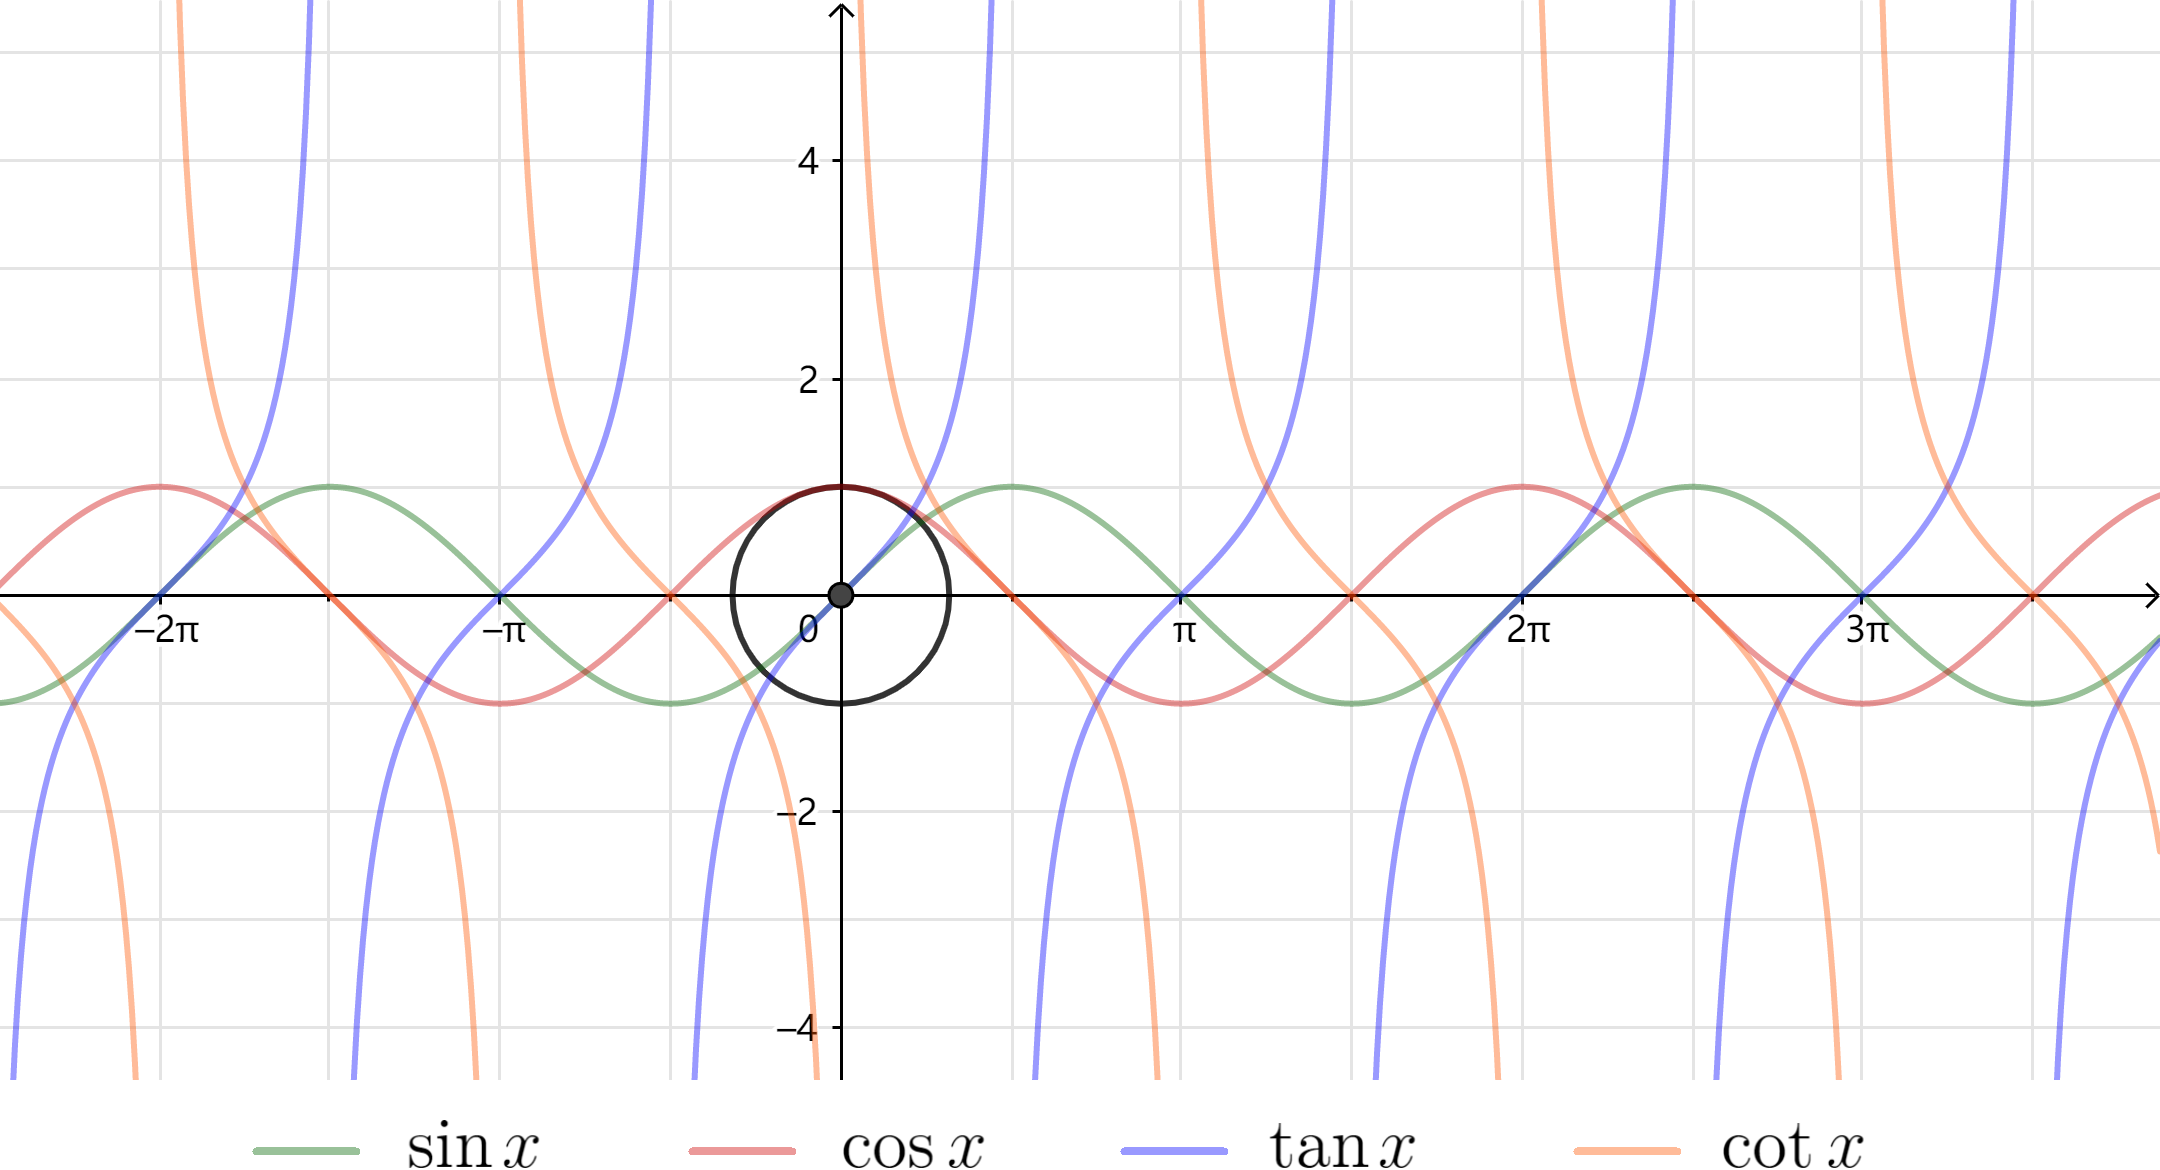
\includegraphics[width=0.96\textwidth]{三角函数1.png}
\end{figure}

这里我们使用\textbf{弧度制}代替角度制。也就是说,我们的自变量不再是角度,而是弧度,
也就是角度在单位圆中对应的圆心角的弧长。角度和弧度的转换可以用以下公式:
$$ \mbox{\texttt{弧度}} = \mbox{\texttt{角度}} \cdot \frac{\pi}{180}, \quad \mbox{\texttt{角度}} = \mbox{\texttt{弧度}} \cdot \frac{180}{\pi}. $$
比如,$30$角度对应$\frac{30\pi}{180}=\frac{\pi}{6}$弧度,
$90$角度对应$\frac{90\pi}{180}=\frac{\pi}{2}$弧度,
$1$弧度对应$\frac{180}{\pi}\approx 57.3$角度,
$\sqrt{2}$弧度对应$\frac{180\sqrt{2}}{\pi}\approx81.03$角度,等等。

从图中可以看到,正弦函数和余弦函数是有界函数,定义域是$\mathbb{R}$,值域是$[-1,1]$。
正切函数和余切函数是无界函数。正切函数的定义域是$\{x\in\mathbb{R}\,|\,x\neq (k+\frac{1}{2})\pi, \,\,\, k\in\mathbb{Z}\}$,
值域是$[-1,1]$。余切函数的定义域是$\{x\in\mathbb{R}\,|\,x\neq k\pi, \,\,\, k\in\mathbb{Z}\}$。
正弦函数和正切、余切函数是奇函数,余弦函数是偶函数。

此外,对任意实数$x$,任意整数$n$,都有$\sin(x+2n\pi) = \sin{x}$,$\cos(x+2n\pi) = \cos{x}$。
对各自定义域中任意实数$x$,任意整数$n$,都有$\tan(x+n\pi) = \tan{x}$,$\cot(x+n\pi) = \cot{x}$。
我们把这样的函数称为周期函数。
\begin{df}
    给定函数$f$。如果有某个正数$T$,使得其定义域中任何$x$,都满足
    $$ f(x + T) = f(x),$$
    就说$f$是\textbf{周期函数},$T$是$f$的\textbf{周期}。
\end{df}
注意到,如果$T$是周期函数$f$的周期,那么$2T$、$3T$、$4T$……都是$f$的周期。
$f$所有周期中若有最小的,就称它为$f$的最小周期,简称“$f$的周期是$T$”。
若不存在最小周期,就说$f$的周期为$0$。常函数是一种特殊的周期函数,任何正数$T$都是它的周期,
我们说常函数的周期是$0$。另一个例子是所谓的\textbf{示理函数}$h$,它的定义是:
$$
h(x) = \left\{
        \begin{array}{cc}
        1 & \mbox{如果}x\in\mathbb{Q} \\
        0 & \mbox{如果}x\notin\mathbb{Q} 
        \end{array}
    \right.
$$
任何有理数$r>0$都是$h$的周期:如果$x$是有理数,那么$x+r$也是有理数,于是$h(x+r) = 1 = h(x)$;
如果$x$是无理数,那么$x+r$也是无理数,于是$h(x+r) = 0 = h(x)$。

正弦和余弦函数的周期都是$2\pi$。正切和余切函数的周期都是$\pi$。

下面来研究三角函数的增减规律。由于三角函数是周期函数,只需要研究一个周期内的增减即可。
又因为三角函数总是奇函数或偶函数,其增减规律关于原点或$y$轴对称,所以只需要研究半个周期。
也就是说,对于正弦函数和余弦函数,我们只需研究区间$[0, \,\,\pi]$;对于正切函数,
只需研究区间$[0, \,\,\frac{\pi}{2})$;对于余切函数,只需研究区间$(0, \,\,\frac{\pi}{2}]$。

我们学习过正弦与余弦函数、正切与余切函数的关联。这里仅举几例:
\begin{align}
    \sin{\left(\frac{\pi}{2} - x\right)} &= \cos{x} \notag \\
    \sin{\left(x + \frac{\pi}{2}\right)} &= \cos{x} \notag \\
    \tan{\left(\frac{\pi}{2} - x\right)} &= \cot{x} \notag     
\end{align}

\begin{wrapfigure}[6]{r}{0.52\textwidth} %this figure will be at the right
    \vspace{-35pt}
    \flushright
    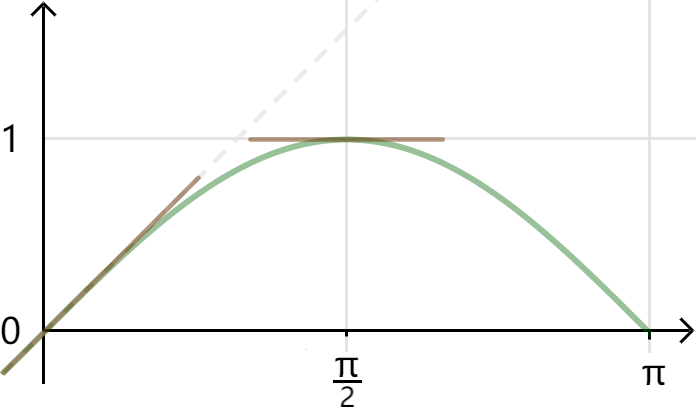
\includegraphics[width=0.5\textwidth]{三角函数2.png}
\end{wrapfigure}

这些关联关系可以让我们在不同的三角函数之间转换,从不同的角度看待问题。
比如,根据第二个公式,正弦函数在区间$[0, \,\,\pi]$上的图像和余弦函数在$[-\frac{\pi}{2}, \,\,\frac{\pi}{2}]$
上的图像是一样的。根据第三个公式,正切函数和余切函数关于直线$x = \frac{\pi}{4}$对称。

现在来看正弦函数在区间$[0, \,\,\pi]$上的图像。

%%% TODO 正弦在区间$[0, \,\,\pi]$上的图像

可以看到,正弦函数的图像总在直线$y = x$下方。在$x = 0$附近,函数值$\sin(x)\approx x$,但随着$x$增大,
$x$的正弦值增大得比$y=x$慢,到了$x=\frac{\pi}{2}$时不再继续增大,而逐渐减小,最终在$x=\pi$时再次变成$0$。

正弦函数是奇函数,所以区间$[-\pi, \,\,0]$上的函数图像与$[0, \,\,\pi]$上的图像关于原点对称。
查看整个周期$[-\pi, \,\,\pi]$,正弦函数在$[-\pi, \,\,-\frac{\pi}{2}]$上严格单调递减;
然后在$[-\frac{\pi}{2}, \,\,\frac{\pi}{2}]$上严格单调递增,又在$[\frac{\pi}{2}, \,\,\pi]$上严格单调递减。
用变化表可以概括为:

\begin{figure}[h] %this figure will be at the right
    % \vspace{-4pt}
    \centering
    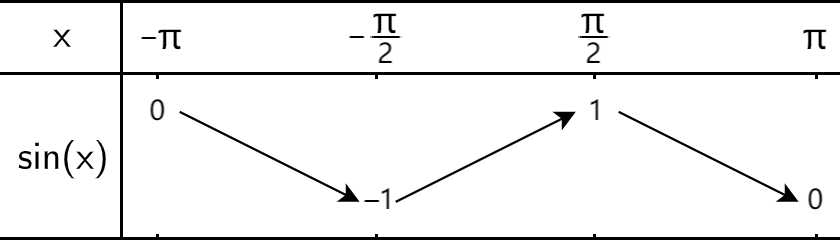
\includegraphics[width=0.63\textwidth]{三角函数变化表1.png}
\end{figure}

余弦函数的增减规律和正弦函数几乎一样。发生在正弦函数$x=x_0$处的事情,
在余弦函数$x=x_0-\frac{\pi}{2}$处发生。因此,在周期区间$[-\pi, \,\, \pi]$上,
余弦函数的增减规律可以用以下变化表概括:

\begin{figure}[h] %this figure will be at the right
    % \vspace{-4pt}
    \centering
    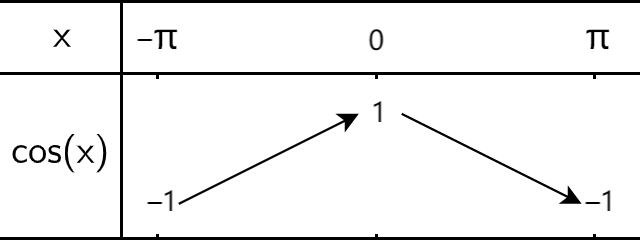
\includegraphics[width=0.48\textwidth]{三角函数变化表2.png}
\end{figure}

正切函数在单个周期内严格单调递增,但在整个定义域中并不是单调函数。
同样,余切函数在单个周期内严格单调递减,但在整个定义域中并不是单调函数。

\section{复合函数和反函数}

设有映射$f$将出发集$A$中元素逐个对应到到达集$B$中元素,又有映射$g$将$f$在$B$中的目标再次对应到集合$C$中元素,
那么我们可以定义两者的\textbf{复合}:
\begin{align}
    g\circ f : \,\,\, A &\rightarrow C \notag \\
    x &\mapsto g(f(x)) \notag
\end{align}

如果$A$、$B$、$C$都是数集,我们就说函数$f$和$g$复合成为$g\circ f$。
要使得映射的复合有意义,$f$的值域$\mathcal{V}_f$应该是$g$的定义域$\mathcal{D}_g$的子集。
这样我们才能把$f(x)$对应到$C$中。如果$\mathcal{V}_f$超出了$\mathcal{D}_g$的范围,
那么我们可以“缩小”$f$的定义域$\mathcal{D}_f$,即找到$\mathcal{D}_f$的子集$\mathcal{D}'$,
使得$f(\mathcal{D}')\subseteq \mathcal{D}_g$。

要注意的是,出于书写习惯,不少人会把这个复合映射写成$f\circ g$,因为在我们的认知中,
$A$中元素先经过$f$映射到$B$中,再经过$g$映射到$C$中。不过我们书写函数的时候,自变量在函数符号的右侧,
因此,为了和$g(f(x))$的书写顺序一致,我们把这个复合映射记作$g\circ f$而不是$f\circ g$。

设函数$f:x\mapsto \sqrt{x}$,$g:x\mapsto 2x - 1$。
则复合函数$g\circ f$为$x\mapsto g(f(x)) = 2\sqrt{x} - 1$。
注意到$f$的定义域是$[0, \,\,+\infty)$,值域是$[0, +\infty)$,$g$的定义域是$\mathbb{R}$,
$g\circ f$的定义域是$[0,\,\, +\infty)$。

另一方面,复合函数$f\circ g$为$x\mapsto \sqrt{2x - 1}$。由于$g$的定义域和值域都是$\mathbb{R}$,
而$f$的定义域是$[0,\,\, +\infty)$,我们需要缩小$g$的定义域,使得$g$的值域落在$f$的定义域中。
也就是说,我们把$g$的定义域缩小到集合:$\{x \,|\, 2x - 1 \in [0, \,\,+\infty)\}$。
这个集合可以化简成$[0.5, \,\,+\infty)$。因此复合函数$f\circ g$为:
\begin{align}
    f\circ g : \,\,\, [0.5,\,\, +\infty) &\rightarrow [0,\,\, +\infty) \notag \\
    x &\mapsto \sqrt{2x - 1} \notag
\end{align}

一般情况下,$g\circ f \neq f\circ g$。甚至,大多数时候,我们无法比较两者,
因为$f$的出发集$g$的到达集不同。只有当$C$和$A$“重合”的时候,我们才有可能比较$g\circ f$和$f\circ g$。

一种特殊情况是$g\circ f$为恒等映射,即对$f$的定义域$\mathcal{D}_f$中的任何元素$x$,总有$g(f(x)) = x$。
我们说这样的$g$是$f$的左逆映射。$f$把某个元素$x$对应到目标函数$y$,而$g$把$f$的目标元素$y$“逆转”为原来的$x$。

要使得$f$的左逆映射$g$有定义,我们要求$f$的定义域$\mathcal{D}_f$等于$g$的值域$\mathcal{V}_g$,
$g$的定义域$\mathcal{V}_g$包含$f$的值域$\mathcal{V}_f$。
且对任意$\mathcal{D}_f$中元素$a \neq b$,$f(a) \neq f(b)$。可以想象,如果有$a \neq b$使得$f(a) = f(b)$,
那么$a = g(f(a)) = g(f(b)) = b$,自相矛盾!我们把满足这个条件的$f$称为\textbf{单射}。

举例来说,函数$f: \,\,x \mapsto \sqrt{x}$是单射,它的定义域是非负实数集合。
可以验证,定义在全体实数上的函数$g:\,\, x \mapsto x^2$是它的左逆映射:
$$ \forall \,\, x \geqslant 0, \,\,\, g(f(x)) = \left(\sqrt{x}\right)^2 = x$$
但$f$不是$g$的左逆映射:$f(g(-1)) = 1$。不过,如果把$g$的定义域缩减到非负实数集合,那么$f$就是$g$的左逆映射了。

%%% 反函数x^2和\sqrt{x} 图像

类似地,如果$f\circ g$是恒等映射,就说$g$是$f$的右逆映射。这时$f$的值域$\mathcal{V}_f$应当等于$g$的定义域$\mathcal{D}_g$。
我们说$f$是$\mathcal{D}_g$上的\textbf{满射}。

按照定义,$g$是$f$的左逆映射,说明$f$是$g$的右逆映射;$g$是$f$的右逆映射,说明$f$是$g$的左逆映射。

如果$g\circ f$是恒等映射,$f\circ g$也是恒等映射,就说$f$和$g$互为逆映射。如果$f$和$g$都是函数,就说它们互为\textbf{反函数}。
这时$f$和$g$既是单射也是满射。
我们把既是单射又是满射的映射称为\textbf{双射}或\textbf{一一对应}。

举例来说,$f: \,\,x\in[0,\,\,+\infty) \mapsto x^2 - 1$是双射。
它的值域是$[-1,\,\,+\infty)$对某个$x\geqslant 0$,记$y = f(x) = x^2 - 1$,
于是$x = \sqrt{y + 1}$。定义函数$g:x\in[-1, \,\,\infty)\mapsto\sqrt{x + 1}$。
那么$\forall x \geqslant 0$,$g(f(x)) = \sqrt{x^2 - 1 + 1} = x$,
$f(g(x)) = \left(\sqrt{x + 1}\right)^2 - 1 = x$。于是$f$和$g$互为反函数。

反函数和本函数有什么联系?我们来看它们在平面直角坐标系中的图像。
设$(x, y)$是$f$的图像上一点,则$y = f(x)$,因此$g(y) = x$。
这说明$(y, x)$是$g$的图像上一点。反过来,如果$(x,y)$是$g$的图像上一点,
则$y = g(x)$,因此$f(y) = x$。这说明$(y, x)$是$f$的图像上一点。
简而言之,交换函数图像上一点的横坐标和纵坐标,就得到它的反函数的图像上一点的坐标。

%%% 反函数x^2 - 1和\sqrt{x + 1} 图像

比如,我们用描点法画出$f: x\in[0,\,\,+\infty) \mapsto x^2 - 1$的图像,
交换每个点的横坐标和纵坐标,得到的新坐标可以描出函数$g:x\in[-1, \,\,\infty)\mapsto\sqrt{x + 1}$的图像。
如果我们作直线$l: y = x$,会发现$f$和$g$的图像关于直线$l$对称。这不难证明:

设$P(a,b)$为$f$图像上一点,则$Q(b,a)$为$g$图像上一点。
过两点的直线为$l':x + y = a + b$。$l'$与$l$垂直,
相交于点$M(\frac{a+b}{2}, \frac{a+b}{2})$,而$|PM| = \frac{|a-b|}{\sqrt{2}} = |QM|$,
因此$l$是$P,Q$中垂线,$P,Q$关于$l$对称。从$g$图像上一点出发,结论相同。这就说明两者图像关于$l$对称。

\begin{sk}
    如果$g$是$f$的左逆映射,并且$g$的定义域$\mathcal{V}_g$等于$f$的值域$\mathcal{V}_f$,能否说明$f$是$g$的左逆映射?为什么?
\end{sk}

\section{反三角函数}

下面来看三角函数的反函数。三角函数是周期函数,所有三角函数$f$都满足$f(x+2\pi) = f(x)$,因此不是单射。
我们退而求其次,只考虑三角函数在部分定义域上的反函数。从上一节可知,反函数的图像和本函数的图像关于直线$l: y = x$对称。
因此,画出三角函数的函数图像后,我们就可以直观地了解反三角函数的图像。

%%% 反正弦函数 图像

首先来看正弦函数($\sin$)的反函数。我们希望选择一个最长的区间,让正弦函数在这个区间上是单射。
常用的区间是$[-\frac{\pi}{2}, \,\, \frac{\pi}{2}]$。
正弦函数在$[-\frac{\pi}{2}, \,\, \frac{\pi}{2}]$上严格单调递增,从$-1$增长到$1$。我们把正弦函数在这个区间上的部分记作$\underline{\sin}$:
\begin{align}
     \underline{\sin} : [-\frac{\pi}{2}, \,\, \frac{\pi}{2}] &\rightarrow [-1,\,\, 1]\notag \\
                                                           x &\mapsto \sin{x} \notag
\end{align}
画出它的图像,按照直线$l: y = x$作对称,就得到它的反函数,称为\textbf{反正弦函数},记作$\arcsin$:
$$ \arcsin : [-1,\,\, 1] \rightarrow [-\frac{\pi}{2}, \,\, \frac{\pi}{2}] . $$
$\arcsin$中的“arc”是“弧长”的意思。$\arcsin$最初表示“把$[-1,\,\, 1]$中的数按正弦函数的反函数对应到单位圆上的弧长”。

举例来说,$\arcsin{1} = \frac{\pi}{2}$,$\arcsin{(-1)} = -\frac{\pi}{2}$,
$\arcsin{0.5} = \frac{\pi}{6}$,$\arcsin{\frac{\sqrt{3}}{2}} = \frac{\pi}{3}$,等等。

从图像中可以看出,反正弦函数也是严格单调递增的函数。它的定义域是$[-1,\,\, 1]$、值域是$[-\frac{\pi}{2}, \,\, \frac{\pi}{2}]$。
$\underline{\sin}$是奇函数,因此,反正弦函数也是奇函数。$x > 0$时,反正弦函数
总在直线$l$上方,增长越来越快;
$x < 0$时,反正弦函数总在直线$l$下方,增长越来越慢。

反正弦函数的定义域是正弦函数的值域。因此,$\sin{(\arcsin{x})} = x$对$[-1,\,\, 1]$中的数总成立。
但反正弦函数的值域只是正弦函数的定义域的真子集,因此,$\arcsin{(\sin{x})} = x$只对$[-\frac{\pi}{2}, \,\, \frac{\pi}{2}]$中的数成立。

再来看余弦函数的反函数。由$\cos{x} = \sin(x+\frac{\pi}{2})$可知,余弦函数的图像可以看作正弦函数的图像按向量$\left(-\frac{\pi}{2}, 0\right)$
平移的结果。因此,我们可以选择$[-\pi, \,\, 0]$作为研究区间。由于余弦函数是偶函数,我们也可以选择$[0,\,\,\pi]$作为研究区间。
常用的区间是$[0,\,\,\pi]$。余弦函数在$[0,\,\,\pi]$上严格单调递减,从$1$减少到$-1$。我们把余弦函数在这个区间上的部分记作$\underline{\cos}$:
\begin{align}
    \underline{\cos} : [0,\,\,\pi] &\rightarrow [-1,\,\, 1]\notag \\
                                                          x &\mapsto \cos{x} \notag
\end{align}
画出它的图像,按照直线$l: y = x$作对称,就得到它的反函数,称为\textbf{反余弦函数},记作$\arccos$:
$$ \arccos : [-1,\,\, 1] \rightarrow [0,\,\,\pi] . $$

%%% 反余弦函数 图像

从图像中可以看出,反余弦函数也是严格单调递减的函数。它的定义域是$[-1,\,\, 1]$、值域是$[-\frac{\pi}{2}, \,\, \frac{\pi}{2}]$。
$x < 0$时,反余弦函数总大于$\frac{\pi}{2}$,减少得越来越慢;$x > 0$时,反余弦函数总小于$\frac{\pi}{2}$,减少得越来越快。

举例来说,$\arccos{1} = 0$,$\arccos{0} = \frac{\pi}{2}$,
$\arccos{(-1)} = \pi$,$\arccos{0.5} = \frac{\pi}{3}$,$\arccos{\frac{\sqrt{3}}{2}} = \frac{\pi}{6}$,等等。

反余弦函数的定义域是余弦函数的值域。因此,$\cos{(\arccos{x})} = x$对$[-1,\,\, 1]$中的数总成立。
但反余弦函数的值域只是余弦函数的定义域的真子集,因此,$\arccos{(\cos{x})} = x$只对$[0,\,\,\pi]$中的数成立。

接下来看正切函数的反函数。正切函数的最小正周期是$\pi$,在$(-\frac{\pi}{2}, \,\, \frac{\pi}{2})$上严格单调递增。
我们把正切函数在这个区间上的部分记作$\underline{\tan}$:
\begin{align}
    \underline{\tan} : (-\frac{\pi}{2}, \,\, \frac{\pi}{2}) &\rightarrow \mathbb{R} \notag \\
                                                          x &\mapsto \tan{x} \notag
\end{align}
画出它的图像,按照直线$l: y = x$作对称,就得到它的反函数,称为\textbf{反正切函数},记作$\arctan$:
$$ \arctan : \mathbb{R} \rightarrow (-\frac{\pi}{2}, \,\, \frac{\pi}{2}) . $$

%%% 反正切函数 图像

从图像中可以看出,反正切函数也是严格单调递增的函数。它的定义域是$\mathbb{R}$、值域是$(-\frac{\pi}{2}, \,\, \frac{\pi}{2})$。
$\underline{\tan}$是奇函数,因此,反正切函数也是奇函数。
$x > 0$时,反正切函数总大于$0$,增长越来越慢;$x < 0$时,反正切函数总小于$0$,增长越来越快。

举例来说,$\arctan{0} = 0$,$\arctan{1} = \frac{\pi}{4}$,
$\arctan{(-1)} = -\frac{\pi}{4}$,$\arctan{\sqrt{3}} = \frac{\pi}{3}$,$\arctan{\frac{\sqrt{3}}{3}} = \frac{\pi}{6}$,等等。

反正切函数的定义域是正切函数的值域。因此,$\tan{(\arctan{x})} = x$对任何实数总成立。
但反正切函数的值域只是正切函数的定义域的真子集,因此,$\arctan{(\tan{x})} = x$只对$(-\frac{\pi}{2}, \,\, \frac{\pi}{2})$中的数成立。

最后来看余切函数的反函数。余切函数的最小正周期是$\pi$,在$(0, \,\, \pi)$上严格单调递减。
我们把余切函数在这个区间上的部分记作$\underline{\cot}$:
\begin{align}
    \underline{\cot} : (0, \,\, \pi) &\rightarrow \mathbb{R} \notag \\
                                   x &\mapsto \cot{x} \notag
\end{align}
画出它的图像,按照直线$l: y = x$作对称,就得到它的反函数,称为\textbf{反余切函数},记作$\arccot$:
$$ \arccot : \mathbb{R} \rightarrow (0, \,\, \pi) . $$

%%% 反余切函数 图像

从图像中可以看出,反余切函数也是严格单调递减的函数。它的定义域是$\mathbb{R}$、值域是$(0, \,\, \pi)$。
$x < 0$时,反余切函数总大于$\frac{\pi}{2}$,减少得越来越快;$x > 0$时,反余切函数总小于$\frac{\pi}{2}$,减少得越来越慢。

举例来说,$\arccot{0} = \frac{\pi}{2}$,$\arccot{1} = \frac{\pi}{4}$,
$\arctan{(-1)} = \frac{3\pi}{4}$,$\arccot{\sqrt{3}} = \frac{\pi}{6}$,$\arccot{\frac{\sqrt{3}}{3}} = \frac{\pi}{3}$,等等。

反余切函数的定义域是余切函数的值域。因此,$\cot{(\arccot{x})} = x$对任何实数总成立。
但反余切函数的值域只是余切函数的定义域的真子集,因此,$\arccot{(\cot{x})} = x$只对$(0, \,\, \pi)$中的数成立。

\begin{sk}
    \mbox{} \\
    \indent 1. 能否找到别的区间来定义反正弦函数?能否找到比$[-\frac{\pi}{2}, \,\, \frac{\pi}{2}]$更长的区间?这样定义的反正弦函数有什么不同?\\
    \indent 2. 能否找到别的区间来定义反余弦函数?能否找到比$[0, \,\, \pi]$更长的区间?这样定义的反余弦函数有什么不同?\\
    \indent 3. 能否找到别的区间来定义反正切函数?能否找到比$(-\frac{\pi}{2}, \,\, \frac{\pi}{2})$更长的区间?这样定义的反正切函数有什么不同?\\
    \indent 4. 能否找到别的区间来定义反余切函数?能否找到比$(0, \,\, \pi)$更长的区间?这样定义的反余切函数有什么不同?\\
    \indent 5. 能否定义正割函数和余割函数的反函数?它们有什么特性?
\end{sk}
\begin{xt}
    \mbox{} \\
    \indent 1. 为什么说“$\underline{\sin}$是奇函数,因此,反正弦函数也是奇函数”?这个说法对一般的函数也成立吗?\\
    \indent 2. 考虑函数$x\mapsto \arcsin{(\sin{x})} - x$,它对哪些实数有定义?画出它在$[-\pi, \,\, \pi]$上的图像。它是周期函数吗?能否将它表示为简单函数和周期函数的和?\\
    \indent 3. 考虑函数$x\mapsto \arctan{(\tan{x})} - x$,它对哪些实数有定义?画出它在$[-\pi, \,\, \pi]$上的图像。它是周期函数吗?能否将它表示为简单函数和周期函数的和?\\
    \indent 4. 考虑函数$x\mapsto \cos(2x - 1)$,它在什么区间上可以定义反函数?如何用反三角函数表示这个反函数?
\end{xt}


\chapter{数列的极限}

\section{极限的基本性质}
我们来考察以下数列:
$$ 0,\,\, \frac{1}{2}, \,\,\frac{2}{3},\,\, \frac{3}{4}, \,\,\frac{4}{5}, \,\,\frac{5}{6}, \cdots $$
它的通项公式是$a_n = \frac{n-1}{n}$。
把数列的前几项在数轴上标出来,我们发现:
随着$n$不断增大,$a_n$不断变大,不断向着$1$靠拢。

数列$\{a_n\}$各项随着$n$增大,不断接近$1$。
虽然数列任一项都不等于$1$,但我们不难产生这样的想法:随着$n$增大,$a_n$的值任意接近于$1$。

怎样严谨地表达这个想法呢?我们使用“有求必应”和“一路全真”的结构,把上面的想法用更具体的方式来描述。
直观来看,我们考察以$1$为中心的区间$[1-r,1+r]$,
无论这个区间多么小,到了一定的$n$以后,所有的$a_n$都会落在这个区间里。

用二元命题$Q(r, n)$表示“$a_n$落在区间$[1-r,1+r]$里”。
用类似“有求必应”的结构,以上的想法可以写成:
$$\forall r > 0, \,\,\, \exists n,  \,\,\, \mbox{使得} \forall \,\, m \geqslant n, \,\,\, Q(r, n)\mbox{成立。}$$
这个结构比“有求必允”结构要求更高。它不仅要求“必允”,而且一旦“允”了,就要求之后“一路全真”。
用表格来表示这个结论:

\begin{figure}[h] %this figure will be at the right
    % \vspace{4pt}
    \centering
    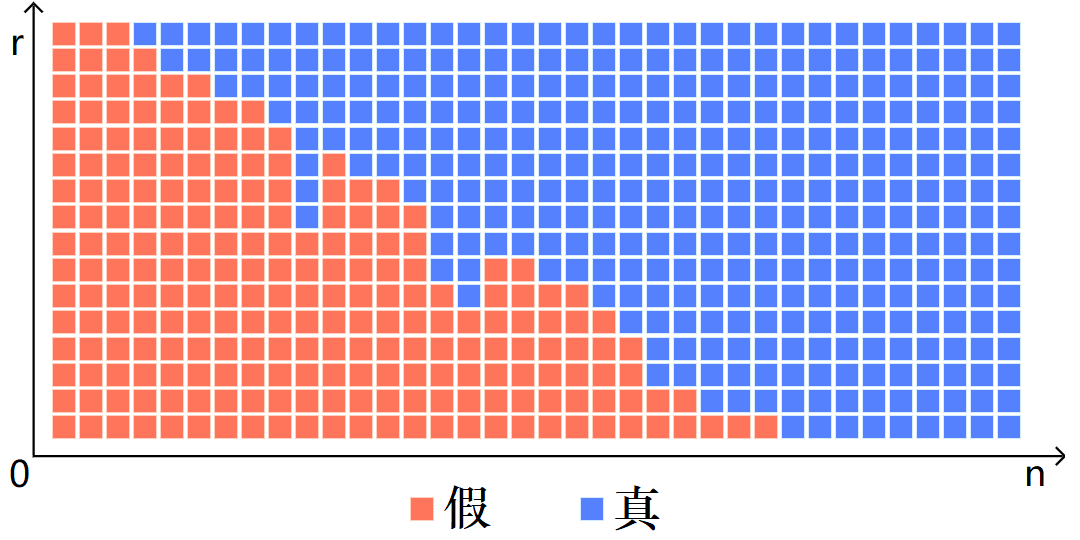
\includegraphics[width=0.64\textwidth]{数列极限2.png}
\end{figure}

每格颜色对应$Q(r, n)$的真假。每一行对应一个正数$r$,每一列对应数列的一个下标$n$。我们的想法是:
不论$r>0$是多少,它对应的行中,$Q(r, n)$必然从某一列起全为真。

我们把$1$称为数列$\{a_n\}$的\textbf{极限}。对一般数列来说,我们定义:
\begin{df}\textbf{数列的极限} \\
设有无穷数列$\{a_n\}$。如果有某个数$x$,使得
$$ \forall r > 0, \,\,\, \exists n,  \,\,\, \mbox{使得} \,\,\, \forall \,\, m \geqslant n, \,\,\, - r \leqslant a_m - x \leqslant r. $$
就说$\{a_n\}$有极限$x$,或$x$是$\{a_n\}$的极限,或$\{a_n\}$趋于$x$,或$\{a_n\}$收敛到$x$,记作
$$\lim_{n\to\infty} a_n = x.$$
数列有极限也称为数列\textbf{收敛},数列没有极限也称数列\textbf{不收敛}。
\end{df}

\begin{figure}[h] %this figure will be at the right
    \vspace{-14pt}
    \centering
    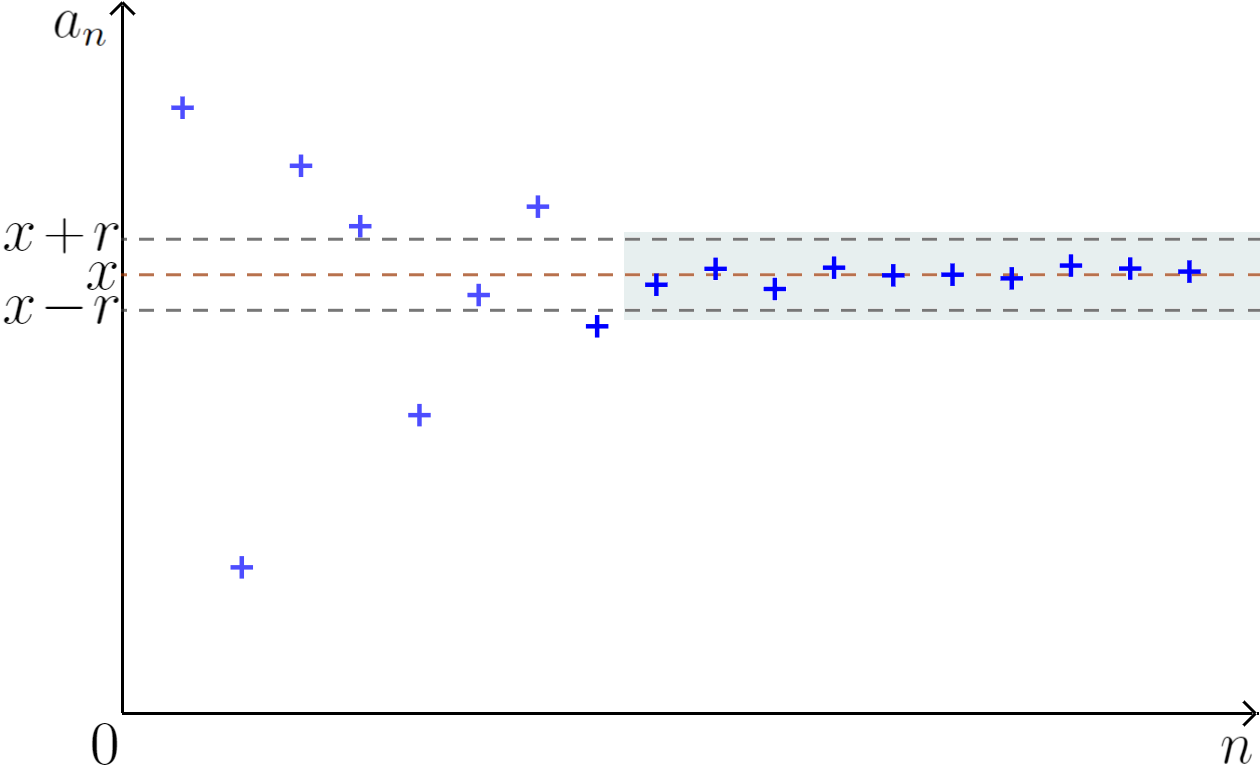
\includegraphics[width=0.54\textwidth]{数列极限1.png}
    \caption*{\texttt{从某一项开始,数列的值总落在区间}$[x-r,x+r]$\texttt{中}}
\end{figure}

\begin{et}
数列$\{a_n\}$的通项是$a_n = \frac{1}{n^2}$,它是否有极限?如果有极限,极限是多少?    
\end{et}
\begin{so}
    $\{a_n\}$每项都是正数。
    $$a_{n} \div a_{n+1} = \frac{1}{n^2} \div \frac{1}{(n+1)^2} = \frac{(n+1)^2}{n^2} = 1 + \frac{2n+1}{n^2} > 1,$$
    所以$\{a_n\}$是单调递减数列。从数轴上看,$\{a_n\}$不断趋近于$0$。猜测它有极限$0$。\\
    设$r>0$,考察区间$[-r,r]$。设$n_r$是大于等于$\frac{1}{\sqrt{r}}$的最小正整数,
    那么,只要$n \geqslant n_r$,就有$n^2 \geqslant n_r^2 \geqslant \frac{1}{r}$,
    于是$0 \leqslant \frac{1}{n^2} \leqslant r$。因此,$\forall r > 0$,$\exists n_r$,
    使得$\forall m \geqslant n_r$,$ -r  \leqslant a_m - 0 \leqslant r$。这说明$\{a_n\}$有极限$0$。    
\end{so}

不难看出,极限是构造出来的。因此,从定义出发,我们可以说某个数是某数列的极限。
反过来,一个数列有极限,它的极限是否只能有一个呢?答案是肯定的。我们可以用反证法来证明。

反设某数列$\{a_n\}$有两个极限$x_1, x_2$。不妨设$x_1 < x_2$。直觉上,$n$足够大的时候,$a_n$在数轴上离$x_1, x_2$都很近,
到两点的距离比$x_2 - x_1$的一半都小,加起来就小于$x_2 - x_1$,于是就产生矛盾了。

具体来说,记$\delta = \frac{x_2 - x_1}{2}$为两点距离的一半。选一个小于$\delta$的正数$r$。
按照极限的定义,有正整数$n_1, n_2$使得:
\begin{align}
    \forall m \geqslant n_1 , \,\,\,& -r \leqslant a_m - x_1 \leqslant r , \notag \\
    \forall m \geqslant n_2 , \,\,\,& -r \leqslant a_m - x_2 \leqslant r . \notag 
\end{align}
于是,选一个比$n_1,n_2$都大的$m$,比如$m=n_1+n_2$,这时$a_m - x_1 \leqslant r$,$x_2 - a_m \leqslant r$。
加起来就得到:
$$x_2 - x_1 \leqslant 2r < 2\delta = x_2 - x_1.$$
矛盾!因此,\textbf{数列如果有极限,只能有一个极限。}

数列的极限,如果存在,是唯一的。我们可以把数列$\{a_n\}$的极限记为$a_\infty$。

设数列$\{a_n\}$有极限$a_\infty$。我们把它每一项减去$a_\infty$,
得到的数列$\{a_n - a_\infty\}$趋于$0$。所以,任何有极限的数列,都可以看做一个趋于$0$的数列加上它的极限。
我们把趋于$0$的数列称为\textbf{无穷小}。任何有极限的数列,都是它的极限加上无穷小。

极限描述了数列的项在“远处”的特征。我们把数列下标超过一定限度后的特征称为数列的\textbf{大体行为}。
有极限的数列,我们可以用极限来刻画数列的大体行为(落在极限“附近”)。
没有极限的数列,大体行为有什么特征呢?

我们来看另一个数列:
$$ 1,\,\,2,\,\,3,\,\,4,\,\,5,\cdots $$
它是正整数数列,通项为$a_n = n$。不难看出,它没有极限。因为对任何实数$x$来说,
令$n_x$为大于$x$的最小正整数,那么从$n_x+1$开始的项都比$x$大至少$1$,
无法落到$x$附近的小区间里面。可以说,随着$n$增大,$a_n$会比任何数都大。

如何严谨描述这个想法呢?我们仍然可以用“有求必应”的结构,把以上想法写成:
$$ \forall x, \,\,\, \exists n, \,\,\,\mbox{使得} \,\,\,\forall \,\, m \geqslant n,,\,\,\, a_m \geqslant x.$$
直观来看,随着$n$增大,从某一项开始,$a_n$会落到数轴任何给定点$x$的右边。
我们把这个性质称为数列\textbf{趋于正无穷大}。同理,可以定义数列\textbf{趋于负无穷大}:
$$\forall x, \,\,\, \exists n, \,\,\,\mbox{使得}\,\,\,\forall \,\, m \geqslant n,,\,\,\, a_m \leqslant x.$$
直观来看,随着$n$增大,从某一项开始,$a_n$会落到数轴任何给定点$x$的左边。

\begin{wrapfigure}[9]{r}{0.33\textwidth} %this figure will be at the right
    \vspace{-48pt}
    \flushright
    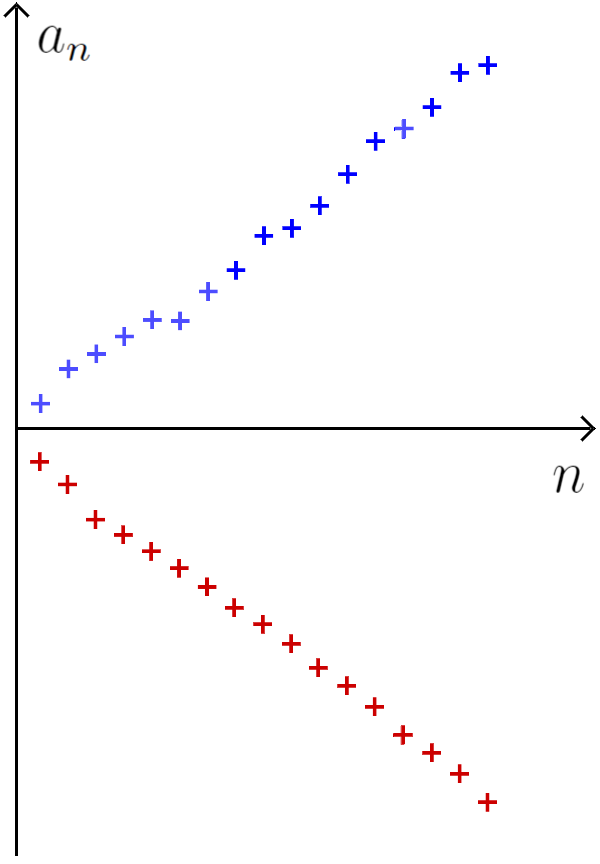
\includegraphics[width=0.32\textwidth]{数列无穷大1.png}
    \caption*{\texttt{趋于无穷大的数列}}
\end{wrapfigure}

我们也把有这两个性质的数列简称为\textbf{正无穷大}和\textbf{负无穷大}。

\begin{et}
    设数列$\{\frac{1}{n}\}$的部分和数列为$\{a_n\}$,证明:$\{a_n\}$趋于正无穷大。
\end{et}
\begin{proof2}
    按照定义,$ a_n = 1 + \frac{1}{2} + \cdots + \frac{1}{n}$。\\
    $a_{n+1} - a_n = \frac{1}{n+1} > 0$,所以$\{a_n\}$单调递增。\\
    对任意实数$x$,我们需要找到相应的$n$,使得$\forall m \geqslant n$,$a_m \geqslant x$。
    由于$\{a_n\}$单调递增,只要某一项$a_n \geqslant x$,它之后的项都大于等于$x$。
    因此,只需要找到$n$使得$a_n \geqslant x$即可。\\
    如果$x \leqslant 1$,那么$n=1$即满足要求。\\
    如果$x > 1$,设$M$是大于$x$的最小整数,考虑$n = 2^{2M}$。下面证明$a_{2^{2M}}>x$。\\
    $$ a_{2^{2M}} = a_{2^0} + \sum_{i=1}^{2M}a_{2^i} - a_{2^{i-1}}.$$
    \begin{align}
        \forall \,\, i\in[1\ldots 2M],\,\,\, a_{2^i} - a_{2^{i-1}} &= \frac{1}{2^{i-1}+1} + \frac{1}{2^{i-1}+2} + \cdots + \frac{1}{2^{i}} \notag \\
        &\geqslant \frac{1}{2^{i}} + \frac{1}{2^{i}} + \cdots + \frac{1}{2^{i}} \notag \\
        &= \frac{2^{i-1}}{2^{i}} = \frac{1}{2}. \notag
    \end{align}
    $$ \mbox{所以}\quad  a_{2^{2M}} \geqslant a_1 + \frac{1}{2} \cdot (2M - 1) = M + \frac{1}{2} > x. $$
    这就证明$\{a_n\}$趋于正无穷大。
\end{proof2}

\begin{sk}
    \mbox{} \\
    \indent 1. 张三在判定数列$\{a_n\}$的极限时写到:数$x$满足:
    $$ \forall r > 0, \,\,\, \exists n,  \,\,\, \mbox{使得} \forall \,\, m > n \,\,\, \mbox{都有} x - r < a_m < x + r. $$
    \indent 因此$\{a_n\}$有极限$x$。他的说法对吗?\\
    \indent 2. 李四在判定数列$\{a_n\}$的极限时写到:数$x$满足:
    $$ \forall r > 0, \,\,\, \exists n,  \,\,\, \mbox{使得} \forall \,\, m > n \,\,\, \mbox{都有} x - 2r \leqslant a_m \leqslant x + 2r. $$
    \indent 因此$\{a_n\}$有极限$x$。他的说法对吗?\\
    \indent 3. 一般数列除了有极限和趋于正/负无穷大,还可能有什么大体行为?\\
    \indent 4. 单调数列除了有极限和趋于正/负无穷大,还可能有什么大体行为?
\end{sk}

\begin{xt}
    \mbox{} \\
    \indent 1. 以下数列是否有极限?如果有极限,是多少?\\
    \indent\indent 1.1. $\{2^{1-n}\}$ \\
    \indent\indent 1.2. $\{(-1)^{n-1}\frac{n+1}{3n+1}\}$ \\
    \indent\indent 1.3. $\{1 - \frac{1}{n^3+1}\}$ \\
    \indent 2. 以下数列是否趋于无穷大?\\
    \indent\indent 2.1. $\{2^{n}\}$ \\
    \indent\indent 2.2. $\{n^2\}$ \\
    \indent\indent 2.3. $\{\frac{2^n}{n^2}\}$\\
    \indent 3. 定义:无穷数列$\{a_n\}$的子列是指从$\{a_n\}$的项中抽取一部分得到的无穷数列。如果数列$\{a_n\}$趋于$x$(趋于正/负无穷大),证明:$\{a_n\}$的任何子列趋于$x$(趋于正/负无穷大)。
\end{xt}

\section{极限的运算}
我们已经学习了数列的运算。数列之间可以做加法、减法、乘法。
如果数列$\{a_n\}$、$\{b_n\}$有极限,它们的和、差、乘积是否有极限?
答案是肯定的,并且符合我们的直觉:
\begin{tm}
    若数列$\{a_n\}$趋于$a$,$\{b_n\}$趋于$b$,则
    \begin{align}
        \lim_{n\to\infty} a_n \pm b_n &= a \pm b, \notag \\
        \lim_{n\to\infty} a_n \cdot b_n &= a \cdot b. \notag 
    \end{align}
\end{tm}
特别地,令$\{b_n\}$是常数列,就得到数乘对极限的影响:若数列$\{a_n\}$趋于$a$,则
$$ \forall \,\, t \in \mathbb{R}, \,\,\,  \lim_{n\to\infty} t \cdot a_n = ta. $$
\begin{proof2}
    \mbox{} \\
    首先证明极限的加法:设数列$\{a_n\}$趋于$a$,$\{b_n\}$趋于$b$。按照定义,$\forall r > 0$,
    由于$\frac{r}{2}>0$,总有正整数$n_a, n_b$,使得
    \begin{align}
        \forall \,\, m \geqslant n_a, \,\,\, & - \frac{r}{2} \leqslant a_m - a \leqslant \frac{r}{2}, \notag \\
        \forall \,\, m \geqslant n_b, \,\,\, & - \frac{r}{2} \leqslant b_m - b \leqslant \frac{r}{2}, \notag 
    \end{align}
    因此,
    \begin{align}
        \forall \,\, m \geqslant n_a + n_b, \,\,\, & -r = - \frac{r}{2} - \frac{r}{2} \leqslant a_m + b_m - a - b \leqslant \frac{r}{2} + \frac{r}{2} = r \notag 
    \end{align}
    于是数列$\{a_n\} + \{b_n\}$趋于$a + b$。\\
    接下来证明极限的数乘:设$t$为实数,数列$\{a_n\}$趋于$a$,则数列$\{t\cdot a_n\}$趋于$ta$。
    这样,数列$\{a_n\} - \{b_n\}$可以看作$\{a_n\} + \{-b_n\}$,因而趋于$a - b$。\\
    分两种情况讨论。如果$t=0$,那么$\{t\cdot a_n\} = \{0\}$,显然趋于$0$,也就是$ta$。
    如果$t \neq 0$,按照定义,对$\forall r > 0$,由于$\frac{r}{t} > 0$,总有正整数$n$使得
    $$ \forall \,\, m \geqslant n, \,\,\, a - \frac{r}{t} \leqslant a_m \leqslant a + \frac{r}{t}. $$
    因此
    $$ \forall \,\, m \geqslant n, \,\,\, ta - r \leqslant t\cdot a_m \leqslant ta + r. $$
    这就说明数列$\{t\cdot a_n\}$趋于$ta$。\\
    最后证明极限的乘法:设数列$\{a_n\}$趋于$a$,$\{b_n\}$趋于$b$。按照定义,$\forall r > 0$,
    由于$\sqrt{r}>0$,总有正整数$n_a, n_b$,使得
    \begin{align}
        \forall \,\, m \geqslant n_a, \,\,\, & - \sqrt{r} \leqslant a_m - a \leqslant \sqrt{r}, \notag \\
        \forall \,\, m \geqslant n_b, \,\,\, & - \sqrt{r} \leqslant b_m - b \leqslant \sqrt{r}, \notag 
    \end{align}
    因此
    \begin{align}
        \forall \,\, m \geqslant n_a + n_b, \,\,\, & (a_m - a)(b_m - b) \leqslant \left(\sqrt{r}\right)^2 = r  \notag \\
        & -(a_m - a)(b_m - b) \leqslant \left(\sqrt{r}\right)^2 = r,  \notag \\
        \mbox{即 }\quad & - r \leqslant (a_m - a)(b_m - b) \leqslant r. \notag 
    \end{align}
    这说明数列$\{(a_n - a)(b_n - b)\}$趋于$0$。而$\{b\cdot a_n\}$和$\{a \cdot b_n\}$都趋于$ab$,
    常数列$\{ab\}$也趋于$ab$,所以根据前面证明的极限加减法,数列
    $$\{a_nb_n\} = \{(a_n - a)(b_n - b)\} + \{b\cdot a_n\} + \{a \cdot b_n\} - \{ab\}$$
    趋于$0 + ab + ab - ab = ab$。
\end{proof2}

四则运算中,加法、减法、乘法都可以对数列的极限做运算。那么除法是否可以呢?
具体来说,若数列$\{a_n\}$趋于$a$,$\{b_n\}$趋于$b$,是否有$\{\frac{a_n}{b_n}\}$趋于$\frac{a}{b}$?

显然,$b=0$的时候,$\frac{a}{b}$无定义,所以先考虑$b$不等于$0$的情况。这时答案大致是肯定的。
$\{\frac{a_n}{b_n}\}$趋于$\frac{a}{b}$。
当然,我们要先“剪掉”$\{b_n\}$最开始一些离$b$比较远的项,确保剩下的项都不等于$0$,这样才好定义$\frac{a_n}{b_n}$。
然后可以用类似证明极限乘法的方法,证明$\{\frac{1}{b_n}\}$趋于$\frac{1}{b}$,
这样,$\{\frac{a_n}{b_n}\}$可以看作$\{a_n \cdot \frac{1}{b_n}\}$,因而趋于$\frac{a}{b}$。

如果$b=0$,即数列$\{b_n\}$为无穷小,那么我们需要考虑的问题就更多了。首先考虑$a\neq 0$的情况。
像前面一样,$\{b_n\}$中等于$0$的项会使得$\frac{a_n}{b_n}$无法定义。
所以我们要确保$\{b_n\}$中没有$0$。其次,我们选择一个很小的正数,比如$r=\frac{a}{101}$。
根据定义,存在正整数$N$,使得对所有$n>N$,$|b_n| \leqslant r$、$|a_n - a| \leqslant r$。
于是,$N$以后的项$\frac{a_n}{b_n}$的绝对值总大于等于$\frac{a - r}{r} = 100$。
然而,这时$a_n$和$b_n$的情况还不一样。$a_n$和$a$相近,因此符号不变。$b_n$则可正可负。
因此,$\frac{a_n}{b_n}$的符号是随着$b_n$改变的。也就是说,$N$项以后,$\frac{a_n}{b_n}$或者大于等于$100$,
或者小于等于$-100$。这样的数列显然没有极限。

于是,我们需要再加一个限制:从某一项开始,$\{b_n\}$的项正负号不变。
这样,根据上面的讨论,可以证明,从某一项开始,$\frac{a_n}{b_n}$的正负号保持不变。

注意到,上面的讨论中把$100$改成任意正数$M$,结论不变。所以,我们实际上已经证明,$\frac{a_n}{b_n}$的绝对值趋于正无穷大。
因此,要么从某一项开始,$\frac{a_n}{b_n}$总大于$0$,因此趋于正无穷大;
要么从某一项开始,$\frac{a_n}{b_n}$总小于$0$,因此趋于负无穷大。

最后考虑$a$也是$0$的情况。这种情况下,不论从哪一项开始,$a_n$、$b_n$都可正可负。
这时,$\{\frac{a_n}{b_n}\}$的大体行为取决于$a_n$、$b_n$之间的关系,不再是可以统一处理的问题。
我们把这种情况下的$\{\frac{a_n}{b_n}\}$称为关于数列$\{a_n\}$和$\{b_n\}$的\textbf{不定式}。
关于数列$\{a_n\}$和$\{b_n\}$的不定式是否有极限,极限是什么,要根据具体情况来讨论。

% \begin{sk}
%     \mbox{} \\
%     \indent 1. 如果数列$\{a_n\}$有极限$a$,$\{b_n\}$趋于无穷大,它们的和、差、乘积、商数列是否有极限?是否趋于无穷大?\\
%     \indent 2. 如果数列$\{a_n\}$、$\{b_n\}$都趋于无穷大,它们的和、差、乘积、商数列有什么特性?
% \end{sk}

\begin{xt}
    \mbox{} \\
    \indent 1. 如果数列$\{a_n\}$有极限$a$,$\{b_n\}$趋于无穷大,它们的和、差、乘积、商数列是否有极限?是否趋于无穷大?\\
    \indent 2. 如果数列$\{a_n\}$、$\{b_n\}$都趋于无穷大,它们的和、差、乘积、商数列有什么特性?
\end{xt}

\section{关于数列极限的一些定理}
\subsection{自敛数列}

我们已经了解过有极限的数列和趋于正(负)无穷大的数列。数列的大体行为是否还有别的可能呢?
要讨论数列的大体行为,我们更关注的是数列“往后”的性质。如果以某个正整数下标$N$为界,把数列分为前$N$项和$N$以后的项,那么$N$以后的项对我们研究大体行为来说更重要。
我们把这部分称为数列截断后的\textbf{余列}。数列$\{a_n\}$第$N$项以后的项($a_{N+1}, a_{N+2}, \cdots$)称为$\{a_n\}$的$N$\textbf{项余列},记作$\{a_n\}_{n>N}$。
任何数列在正整数$N$处截断,都能得到一个长度为$N$的有穷数列,以及一个$N$项余列。

我们引入一个新的性质:
\begin{df}
    如果随着$N$增大,数列$\{a_n\}$的$N$项余列中,各项之间的差任意小,就说数列$\{a_n\}$是\textbf{自敛}的(或者说$\{a_n\}$有\textbf{自敛性})。
    具体来说,如果对任意正数$r$,都存在正整数$N$,使得对$\{a_n\}_{n>N}$中任何两项$a_k, a_m$,都有$|a_k - a_m| \leqslant r$,就说数列$\{a_n\}$是\textbf{自敛}的。
\end{df}
顾名思义,自敛的数列,指数列的项会逐渐相互靠近,自相收敛到一起。不难看出,\textbf{有极限的数列,总是自敛的},
因为它的项会逐渐趋于它的极限,于是互相靠近,收敛到一起。
反之是否成立呢?对于实数来说,这个性质是成立的。我们把这个性质称为实数的\textbf{致密性}或\textbf{完备性}。

\begin{po}\textbf{实数完备性}
    任何自敛的实数数列总有极限,极限为实数。
\end{po}

我们可以从另一个角度来理解这个性质。考虑数列$\{a_n\}$:
$$ a_1 = 1, \quad \forall \,\, n \in \mathbb{Z}^+, \,\,\, a_{n+1} = \frac{a_n}{2} + \frac{1}{a_n} $$
$\{a_n\}$的项是有理数四则运算的结果,所以总是有理数。用归纳法可以证明,$1 < a_n < 2$总成立。此外可以验证:
$$ a_{n+1} - \sqrt{2} = \frac{(a_n - \sqrt{2})^2}{2a_n},$$
因此,
$$ |a_{n+1} - \sqrt{2}| = \frac{|a_n - \sqrt{2}|}{2|a_n|} \cdot |a_n - \sqrt{2}| < \frac{2 - \sqrt{2}}{2} \cdot |a_n - \sqrt{2}| < 0.3\cdot |a_n - \sqrt{2}|. $$
这说明总有$|a_n - \sqrt{2}| < (0.3)^{n-1}$。于是$\{a_n\}$趋于$\sqrt{2}$。然而,$\sqrt{2}$并不是有理数。这说明有理数集合并不是致密的。
一列有理数互相靠近,自相收敛,但它们最终收敛的结果,是不属于有理数集合的“空隙”。

对有理数来说,“数列的极限”这个概念是不完备的:我们没法只通过有理数来讨论有理数列的极限。

而实数的完备性说明,如果一列实数互相靠近,不断聚拢到一起,那么最终总能收敛到某个实数,而非某个不属于实数集合的“新数”。

实数的致密性(完备性)是实数集合的根本性质,是对日常生活中“长度”概念进行抽象得到的必然结果:我们认为任意的长度都是存在的,直尺上不可能有两点之间没有长度。
即便由于测量工具的局限,我们无法精确测量物体的长度,我们也相信,物体的长度是一个真实存在的数,可以无限逼近。
\textbf{实数是人类在自身尺度下对世界的朴素认知的抽象}。

\begin{xt}
    \mbox{}\\
    \indent 1.已知数列的通项公式或递推公式,证明数列是自敛数列:\\
    \indent 1.1. $\{\frac{1}{n^2}\}_{n\in\mathbb{Z}^+}$\\
    \indent 1.2. $a_1 = 2, \quad \forall \,\, n\in\mathbb{Z}^+, \,\,\, a_{n+1} = \frac{a_n}{2} + \frac{1}{2a_n}.$\\
    \indent 1.3. $\left\{\frac{\sin(n)}{n}\right\}_{n\in\mathbb{Z}^+}$ \\
    \indent 2. 证明:有极限的数列,总是自敛数列。
\end{xt}

\subsection{数列的确界}
单调数列是一种简单的数列,单调递增数列中,每一项都大于等于前面的项;单调递减数列中,每一项都小于等于前面的项。单调数列的大体行为有哪些呢?

以单调递增数列为例。我们已经见过有极限的单调递增数列和趋于正无穷大的单调递增数列。除此以外,还有别的可能性吗?

我们用“是否有上界”来分类讨论。如果单调递增数列$\{a_n\}$没有上界,则按照定义,对任何数$M$,都存在正整数$N$,使得$a_N > M$。
由于$\{a_n\}$单调递增,$n > N$时,$a_n$也大于$M$。因此,$\{a_n\}$趋于正无穷大。

如果如果单调递增数列$\{a_n\}$有上界,即有某个数$M$,
使得$a_n \leqslant M$总成立。由于$a_n$随着$n$增大而增大,可以想象,增大会逐渐变缓乃至停滞。因此,$\{a_n\}$应该收敛于某个不大于$M$的数。

这个数显然在$a_1$和$M$之间。为了找出这个数,设定正整数$k$之后,我们把$M - a_1$这段距离均匀分成$k$份,记每份的大小为$r_k = \frac{M - a_1}{k}$。
从$M$出发,一步步“往$a_1$走”:
$$ M, M - r_k, M - 2r_k, \cdots, M - k r_k = a_1.$$
如果在第$i$步,数列中所有的数都小于$M - (i-1)r_k$,而在第$i+1$步,有某一项$a_{N(k)}$大于等于$M - i r_k$,就停下来,考虑区间$I_k = [M - (i-1)r_k, \,\, M - i r_k]$。

区间$I_k$的长度是$r_k$,而$a_{N(k)}$在$I_k$中。不仅如此,$n>N(k)$时,$a_{N(k)} \leqslant a_n < M - (i-1)r_k$,因此总在$I_k$中。
这说明$\forall m,n\geqslant N(k)$,$|a_m - a_n|$总小于$r_k$。而$r_k$无非是$\frac1k$的常数倍数。因此,对任何正数$r$,我们只要令$k$为大于$\frac{M - a_1}{r}$的正整数,就有
$r_k = \frac{M - a_1}{k} < r$。于是$\forall m,n\geqslant N(k)$,$|a_m - a_n|$总小于$r$。这说明$\{a_n\}$是自敛数列,因此有极限。

综上所述,单调递增数列要么趋于正无穷大,要么有极限。类似可以证明:单调递减数列要么趋于负无穷大,要么有极限。一个简单的判定法则是:
\begin{tm}\textbf{单调收敛定理}
    有上界(下界)的单调递增(递减)数列必然有极限。
\end{tm}
由于单调递增(递减)数列必然有下界(上界)$a_1$,单调收敛定理可以简化为:\textbf{有界单调数列收敛}。我们把有界单调数列的极限称为它的\textbf{确界}。
单调递增数列的极限叫做它的\textbf{上确界},单调递减数列的极限叫做它的\textbf{下确界}。

以单调递增数列来说,如果单调递增数列$\{a_n\}$有上界,设$S_a$为$\{a_n\}$上界的集合,那么上确界$a_\infty$就是其中最小的元素。证明如下:

首先证明$a_\infty \in S_a$。用反证法。反设$a_\infty$不是$\{a_n\}$的上界,则有某个$a_N$大于$a_\infty$,因此其后的项都大于$a_\infty$。即$n > N$时,
$a_n - a_\infty > a_N - a_\infty$。于是,对正数$a_N - a_\infty$来说,没有正整数$m$使得其后的项与$a_\infty$的差都小于等于$a_N - a_\infty$。
这与$\{a_n\}$趋于$a_\infty$矛盾!因此$a_\infty$是$\{a_n\}$的上界。

其次证明$\{a_n\}$的上界中没有比$a_\infty$更小的。仍然用反证法。反设$b \in S_a$是某个比$a_\infty$更小的上界:$b < a_\infty$。于是$a_n \leqslant b$总成立。也就是说,
$$\forall \,\, n, \,\,\, a_\infty - a_n = a_\infty - b + b - a_n \geqslant a_\infty - b.$$
这说明$\{a_n\}$所有的项和$a_\infty$的差都大于等于固定的正数$a_\infty - b$。于是,对正数$r = \frac{a_\infty - b}{2}$来说,没有正整数$m$使得其后的项与$a_\infty$的差都小于等于$r$。
这与$\{a_n\}$趋于$a_\infty$矛盾!因此$\{a_n\}$的上界中没有比$a_\infty$更小的。

综上所述,$a_\infty$是$S_a$中最小的元素。

同样地,如果单调递减数列$\{a_n\}$有下界,那么下确界$a_\infty$就是其中最大的元素。

\chapter{二项式}

我们知道整式分为单项式和多项式,而多项式中最简单的是二项式。
很多实际问题中,我们可以把感兴趣的对象分成两部分的和,
写成$a+b$的形式,这使得数学家对表达式$(a+b)^n$展开了研究。

\section{杨辉三角形}

$(a+b)^n$展开是什么样子?$n=1,2,3$时,我们知道,
\begin{align}
 (a + b)^1 &= a + b \notag \\
 (a + b)^2 &= a^2 + 2ab + b^2 \notag \\
 (a + b)^3 &= a^3 + 3a^2b + 3ab^2 + 3b^3 \notag 
\end{align}

继续让$n=4,5,6$,可以算出
\begin{align}
 (a + b)^4 &= a^4 + 4a^3b + 6a^2b^2 + 4ab^3 + b^4 \notag \\
 (a + b)^5 &= a^5 + 5a^4b + 10a^3b^2 + 10a^2b^3 + 5ab^4 + b^5 \notag \\
 (a + b)^6 &= a^6 + 6a^5b + 15a^4b^2 + 20a^3b^3 + 15a^4b^2 + 6a^5b + b^6 \notag 
\end{align}

观察这些式子中各项,我们可以发现一些规律。

首先,$(a+b)^n$的展开式一共有$n+1$项。将它们按$a$的幂次从高到低排列,
第$k$项可以写成$a^kb^{n-k}$乘以常数系数的形式。
也就是说,$(a+b)^n$的展开式恰好包含了$a,b$构成的所有$n$次齐次式,没有遗漏。

其次,首项$a^n$和末项$b^n$的系数总是$1$。此外,每项前的系数有对称性。
$a^kb^{n-k}$的系数和$a^{n-k}b^k$的系数总相同。
我们把这些系数排列成如下三角形的样子(第一行代表$(a+b)^0=1$的系数$1$):

\begin{figure}[h] %this figure will be at the right
    \vspace{-14pt}
    \centering
    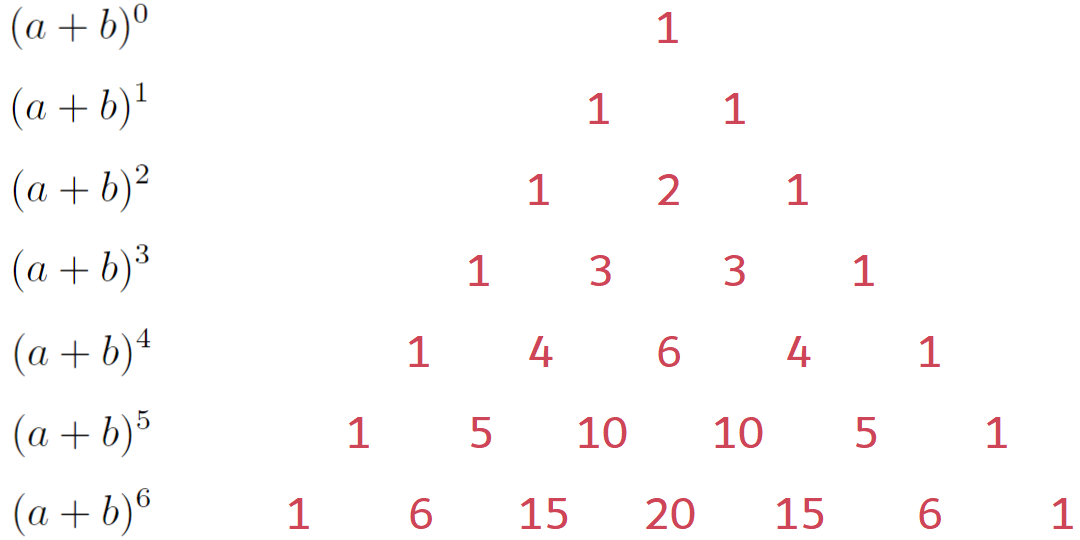
\includegraphics[width=0.72\textwidth]{二项式1.png}
\end{figure}

可以看到,每一行相邻的两个系数之和,等于下一行位于它们“中间”的数。
例如,第$5$行第$2$个数$4$和第$3$个数$6$的和等于$10$,也就是第$6$行第$3$个数。

继续算出$n=7,8$时$(a+b)^n$的系数,可以验证,以上规律仍然成立。

公元$1261$年,南宋数学家杨辉所著的《详解九章算术》中就出现了这个三角数阵,
我们把它称为\textbf{杨辉三角形}。使用杨辉三角形,我们可以方便地查出$(a+b)^n$各项的系数。
下面我们归纳法证明以上规律。

记$(a+b)^n = \sum_{k=0}^n w_{k,n} a^k b^{n-k}$,其中$w_k$是各项系数。
设立命题$P(n)$:$w_{0,n}=w_{n,n}=1$;$\forall k\in[1\ldots n-1]$,$w_{k,n} = w_{k,n-1} + w_{k-1,n-1}$。

$n=2$时,$w_{1,2} = 2 = 1 + 1 = w_{1,1} + w_{0,1}$。因此$P(2)$为真。

若$P(n)$对某个自然数$n\geqslant 2$为真,根据归纳假设,
\begin{align}
 (a+b)^{n+1} &= (a+b)\cdot(a+b)^n = (a+b)\cdot\left(\sum_{k=0}^n w_{k,n} a^k b^{n-k}\right) \notag \\
  &= \sum_{k=0}^n w_{k,n} a^{k+1} b^{n-k} + \sum_{k=0}^n w_{k,n} a^k b^{n-k+1} \notag \\
  &= w_{n,n}a^{n+1} + \sum_{k=0}^{n-1} w_{k,n} a^{k+1} b^{n-k} + \sum_{k=1}^n w_{k,n} a^k b^{n-k+1} + w_{0,n}b^{n+1} \notag \\
  &= a^{n+1} + \sum_{k=1}^{n} w_{k-1,n} a^{k} b^{n-k+1} + \sum_{k=1}^n w_{k,n} a^k b^{n-k+1} + b^{n+1}\notag \\
  &= a^{n+1} + \sum_{k=1}^{n} (w_{k-1,n} + w_{k,n}) a^{k} b^{n-k+1} + b^{n+1} \notag
\end{align}
因此$w_{0,n+1}=w_{n+1,n+1}=1$;$\forall k\in[1\ldots n]$,$w_{k,n+1} = w_{k,n} + w_{k-1,n}$。
于是$P(n+1)$为真。因此,对任何为真大于等于$2$的自然数,$P(n)$为真。

根据以上递推公式,我们可以算出杨辉三角形任一行的数。以此为系数,我们可以写出任何$(a+b)^n$的展开式。

\section{二项式定理}

设$n=100$,我们想知道$(a+b)^n$的展开式。仅仅根据递推公式,为了算出$(a+b)^n$,
我们要先推出前$100$行。这样的计算太繁琐了。我们希望对每个系数有直接了解。能否有计算指定系数的“通项公式”?

我们先从比较小的$n$开始找规律。展开$(a+b)^2$的时候,我们根据分配律,得到
$$ (a+b)^2 = a\cdot a + b\cdot a + a\cdot b + b\cdot b. $$
然后把$ab$和$ba$合并同类项。展开$(a+b)^3$的时候,我们根据分配律,得到
\begin{align}
 (a+b)^3 &= a\cdot a\cdot a + b\cdot a\cdot a + a\cdot b\cdot a + b\cdot b\cdot a\notag \\
  &+ a\cdot a\cdot b + b\cdot a\cdot b + a\cdot b\cdot b + b\cdot b\cdot b \notag 
\end{align}
然后把$baa$、$aba$、$aab$合并同类项,得到$3a^2b$;把$bba$、$bab$、$abb$合并同类项,得到$3ab^2$。

一般来说,展开$(a+b)^n$时,我们已经知道所有的项都是$a^kb^{n-k}$乘以相应系数的形式,
其中的$a$和$b$来自于每次使用分配律时选择$a$还是$b$,而系数是所有相应选择的方法数。
具体来说,我们可以认为,展开$(a+b)^n$时,我们从$n$个连乘的$a+b$中不断选择,
把$n$次选择的结果乘起来,然后合并到某个$a^kb^{n-k}$中,成为它的系数中的“$1$”。
所有的“$1$”加起来,就变成了展开式中$a^kb^{n-k}$的系数。

例如,展开$(a+b)^6$时,我们已经知道有$a^2b^4$这一项($k=2$)。它的系数是在$6$个$a,b$中选择$2$次$a$、$4$次$b$的方法数,即组合数$C_6^2$。
于是,$(a+b)^6$的展开式中,$a^2b^4$这一项的系数是$C_6^2 = 15$。

对特定的$k$来说,$a^kb^{n-k}$的系数来自于我们展开时选择了$k$次$a$、$n-k$次$b$。
因此,$a^kb^{n-k}$的系数就等于选出$k$个$a$和$n-k$个$b$的方法数。它等于组合数$C_n^k$。
也就是说,$(a+b)^n$的展开式中,$a^kb^{n-k}$的系数为$C_n^k$。这个系数叫做\textbf{二项式系数}。
我们可以完整地写出$(a+b)^n$的展开式:
$$(a+b)^n = \sum_{k=0}^n C_n^k a^kb^{n-k} = \sum_{k=0}^n \frac{n!a^kb^{n-k}}{k!(n-k)!} .$$
这个结论称为\textbf{二项式定理},右边的式子称为$n$次二项展开式。其中为了方便,
约定$C_n^0 = \frac{n!}{0!n!} = 1 = C_n^n$。

组合数是二项式展开中的系数,因此,可以用二项式定理反过来推导出组合数的一些基本性质。
比如,由前面的结论可知:
$$C_n^k = C_n^{n-k}, \quad C_{n+1}^k = C_n^k + C_n^{k-1}.$$
又如,令$a=b=1$,可得到:
$$\sum_{k=0}^n C_n^k = 2^n.$$
令$a=-1$、$b=1$,可得到:
$$\sum_{k=0}^n (-1)^k C_n^k = 0.$$

观察杨辉三角形,还可以发现二项式系数的性质:从$C_n^0=1$起,随着$k$增大,
$C_n^k$先是不断增大,然后不断减小,最终回到$C_n^n = 1$。
$n=2m+1$为奇数的时候,$C_n^m=C_n^{m+1}$是数值最大的;$n=2m$为偶数时,
$C_n^m$是数值最大的。这些性质可以用以下关系式解释:
$$ C_n^k = \frac{n!}{k!(n-k)!} = \frac{n-k+1}{k}\cdot \frac{n!}{(k-1)!(n-k+1)!} = \frac{n-k+1}{k}C_n^{k-1}.$$
$k < n-k+1$的时候,$C_n^k > C_n^{k-1}$;$k > n-k+1$的时候,$C_n^k < C_n^{k-1}$。分水岭是$\frac{n+1}{2}$。

具体来说,$C_n^k$大概有多大呢?我们知道,使得$C_{n}^k$最大的$k$在$n$的一半左右。
使用渐进估计(需要用到较高深的知识,这里不展开介绍)可以知道,
$n$足够大之后,这个系数大致等于$\frac{2^{n}}{\sqrt{2\pi n}}$。
也就是说,所有二项式系数之和大致是最大的二项式系数的$2.5\sqrt{n}$倍。
二次项系数从$1$变成$n$,再变成$\frac{n(n-1)}{2}$,增长越来越慢,
最终在$n$的一半左右达到最大值————大约是$\frac{2^{n}}{\sqrt{2\pi n}}$,然后逐渐变小,最后回到$1$。

\begin{xt}
    \mbox{} \\
    \indent 1. 展开以下二项式:\\
    \indent 1.1. $(a+b)^8$、$(a-b)^{10}$ \\
    \indent 1.2. $(x+1)^7$、$(1-\frac{1}{x})^9$、$(x^2-\frac{1}{x})^5$ \\
    \indent 2. 观察$(1+x)^{2n}$的系数,证明:$\sum_{k=0}^n \left(C_n^k\right)^2 = C_{2n}^n.$ \\
    \indent 3. 观察$a^n = (a-b+b)^n$的系数,证明:
                $$\forall \,\, 0 \leqslant m < n, \,\,\, \sum_{k=m}^n (-1)^{k-m} C_n^kC_k^m = 0.$$
    \indent 4. $7^{103}$模$25$的余数是多少?

\end{xt}

\section{二项式的应用}

二项式在科学研究、生产生活中经常出现,有大量应用。这里举两个简单的例子。

\subsection{二项分布}

我们已经学习过单一实验中的二项分布。比如,抛一枚硬币,硬币正面向上的概率是$p$,
向下的概率是$1-p$,就说实验结果服从系数为$p$的二项分布。现在来看独立重复这个实验的分布。

假设重复抛掷$n$次硬币,任何两次之间互不干扰。这个独立重复实验中,每次抛掷正面向上的概率为$p$,
向下的概率为$1-p$。$n$次抛掷是相互独立的,因此,某$k$次抛掷正面向上,其余$n-k$次抛掷向下的概率是$p^k(1-p)^{n-k}$。
$n$次抛掷中,要使得$k$次抛掷向上,有$C_n^k$种可能,因此,$n$次抛掷中有$k$次正面向上的概率就是$C_n^kp^k(1-p)^{n-k}$,
也就是二项式$(p + 1-p)^n$展开中第$k+1$项。这样的分布称为系数为$p$的$n$次二项分布。
$n$次抛掷的终态有$n+1$个,其分布列为:
\begin{center}
    \begin{tabular}{| p{4em}<{\centering} | p{8em}<{\centering} |}
        \hline
        $\mathbf{k}$ & $\mathbb{P}(\mathbf{k}\mbox{\textbf{次正面向上}})$ \\ [0.5ex] 
        \hline
        $0$ & $C_n^0 p^0(1 - p)^n\quad$ \\  
        \hline
        $1$ & $C_n^1 p^1(1 - p)^{n-1}\,$ \\  
        \hline
        $\vdots$ & $\vdots$  \\    [0.75ex] 
        \hline
        $n-1$ & $C_n^n p^{n-1}(1 - p)^{1}\quad$ \\ 
        \hline
        $n$ & $C_n^n p^n(1 - p)^{0}\quad$ \\ 
        \hline
    \end{tabular}
\end{center}
比如,抛掷$n=20$次硬币,向上概率为$p=0.4$的时候,分布可以用以下直方图表示:

%%% TODO 二项分布 直方图

可以算出,$5$次向上的概率约为$0.0746$,$10$次向上的概率约为$0.1171$,$15$次向上的概率约为$0.0013$。

\begin{xt}
    \mbox{} \\
    独立重复抛掷$15$次硬币,每次抛掷向上的概率是$0.6$
    \indent 1. $3$次向上、$6$次向上、$8$次向上的概率分别是多少?用计算器算出以上概率。\\
    \indent 2. 画出这个实验结果的分布列。\\
    \indent 3. 几次向上的概率最大?
\end{xt}

\subsection{近似计算}
\begin{et}
    已知某合金的长度热膨胀满足半经验公式:$l = l_0(1+\eta\frac{T-T_0}{T_0})^5$,
    原材料长度$l_0=25$厘米,系数$\eta=0.5$。当温度$T$从$T_0=650K$升到$654K$的时候,材料长度增加了多少厘米?将误差保持在$1\%$以内。
\end{et}
\begin{so}
    关键在于计算$(1+\eta\frac{T-T_0}{T_0})^5$。$\eta\frac{T-T_0}{T_0} = \frac{2}{650} \approx 0.00308$。
    因此需要计算
    $$ 1 + 5\cdot 0.00308 + 10\cdot 0.00308^2 + 10 \cdot 0.00308^3 + 5 \cdot 0.00308^4 + 0.00308^5. $$
    我们注意到$0.00308$是一个很小的数,它的平方、立方……只会迅速变得非常非常小。而二项式系数最大不超过$10$,
    因此,上式左起第$3$项开始相对前两项非常小。\\
    由于$5 \cdot 0.00308 = 0.0154$,而$10\cdot 0.00308^2 \approx 0.00009$,
    大概是$0.0154$的千分之六,在$1\%$以内,因此它之后的项就可以忽略了。我们可以说
    $$ (1+\frac{T-T_0}{T_0})^5 \approx 1 + 5\cdot 0.00308 + 10\cdot 0.00308^2 = 1.0155 $$
    因此,升温后材料长度约为$25\cdot 1.0155 = 25.387$厘米,增加了$0.387$厘米。
    精确计算的结果是$0.38699\dots$厘米,可以看出误差在$1\%$以内,未造成额外误差。   
\end{so}

我们把这样的问题称为\textbf{微扰估计问题},即估计一个形如$(1+x)^n$的式子在$x$很接近$0$的时候大约和$1$差多少。
其中$x$一般称为扰动项。

考虑$(1+x)^n$的展开式。前文已经介绍过,展开式中第$k+1$项$C_n^kx^k$的“大小”大约是
$\frac{2^{n}x^k}{\sqrt{2\pi n}}$。而$x$接近$0$的时候,二项式系数增长比起幂函数要“慢”,
即$x^k$远比$2^n$小。因此,展开式中$x$次数越高的项,越快速接近$0$,在$x$次数较低的项前面,小得可以忽略。

比如,在前面的例子里,$x\approx 0.003$,$x^1$就已经远远小于$2^5$,
$$C_5^2x^2 = \left(\frac{C_5^2}{C_5^1}x\right)\cdot C_5^1x^1$$
括号中的$\frac{C_5^2}{C_5^1}x$远小于$1$,因此$C_5^2x^2$远小于$C_5^1x^1$,
其后的$C_5^3x^3$、$C_5^4x^4$、$C_5^5x^5$更是如此。于是,我们可以根据精度要求,适当舍掉靠后的大部分项,
只保留靠前$x$次数较低的项,快速估计出近似值。

实践中,我们只保留前一到两项,精度不够时,再逐步尝试。比如先计算$1 + C_n^1x = 1 + nx$,
再计算$1 + C_n^1x + C_n^2x^2 = 1 + nx + \frac{n(n-1)}{2}x^2$。如果两者之差在精度要求的误差范围内,
就可以用后一个作为估计结果。
\begin{et}
    计算$(1 - 0.0082)^{14}$,相对误差在$1\%$以内。
\end{et}
\begin{so}
    $n=14$,$x=-0.0082$,计算$1 + nx$和$1 + nx + \frac{n(n-1)}{2}x^2$的值,分别得到$0.8852$和$0.8913$。两者之差为$0.0061$,小于$1\%$,因此认为精度已达到要求,取$0.8913$为估计结果。经验证,精确结果为$0.89112\dots$,相对误差在$1\%$以内。
\end{so}
\begin{et}
    计算$1.9926^{19}$,相对误差在$1\%$以内。
\end{et}
\begin{so}
    将问题转化为求$2^{19}\cdot(1-\frac{2-1.9926}{2})^{19}$。这时$n=19$,$x = -\frac{2-1.9926}{2} = -0.0037$。计算$1 + nx$和$1 + nx + \frac{n(n-1)}{2}x^2$的值,分别得到$0.9297$和$0.9320$。两者之差为$0.0023$,小于$1\%$,因此认为精度已达到要求。估计结果为$2^{19}\cdot 0.9320=488636.416$。经验证,精确结果为$488632.549\dots$,相对误差在$1\%$以内。
\end{so}

\begin{sk}
    如果某合金的长度热膨胀满足半经验公式:$l = l_0(1+\eta\frac{T-T_0}{T_0})^{0.5}$。原材料长度$l_0=25$厘米,系数$\eta=0.5$。当温度从$400K$升到$450K$时,材料长度如何变化?
\end{sk}

\chapter{不等式}

\section{不等式的基本概念}

我们已经接触过一元一次、一元二次和二元一次不等式。当变量取某些值的时候,不等式成立;
取另一些值的时候,不等式不成立。这样的不等式称为\textbf{条件不等式}。如果无论变量取什么值,不等式都成立,
这样的不等式称为\textbf{绝对不等式}。

先来复习一下不等关系的基本规则:

这些性质基于数的运算法则,对我们熟知的数域:$\mathbb{N}$、$\mathbb{Z}$、$\mathbb{Q}$、$\mathbb{R}$都成立。
此外,从数的运算法则,还可以给出以下的不等关系:
\begin{enumerate}
    \item 任何数的平方大于等于$0$。
    \item 同号的数相乘大于$0$。异号的数相乘小于$0$。
\end{enumerate}

利用这些性质,我们可以得出一些有用的结论,称为常用不等式。

\section{排序不等式}

给定两列数:$a_1 \geqslant a_2 \geqslant \cdots \geqslant a_n$和
$b_1 \geqslant b_2 \geqslant \cdots \geqslant b_n$。它们都按从大到小的顺序排列。
我们把数列$\{a_k\}$中最大的数乘以$\{b_k\}$中最大的数,把$\{a_k\}$中次大的数乘以$\{b_k\}$中次大的数,
以此类推,再全部加起来,把得到的和称为两列数的\textbf{顺序和}:
$$ a_1b_1 + a_2b_2 + \cdots + a_nb_n $$
我们把数列$\{a_k\}$中最大的数乘以$\{b_k\}$中最小的数,把$\{a_k\}$中次大的数乘以$\{b_k\}$中次小的数,
以此类推,再全部加起来,把得到的和称为两列数的\textbf{逆序和}:
$$ a_1b_n + a_2b_{n-1} + \cdots + a_nb_1 $$
按照其它顺序把两列数两两配对(不重复也不遗漏),加起来的和,称为两列数的\textbf{乱序和}:
$$ a_1b_{g(1)} + a_2b_{g(2)} + \cdots + a_nb_{g(n)} $$
其中$g$是某个$[1\dots n]$到自身的双射。

\begin{tm}\textbf{排序不等式}\\
    两列数的顺序和大于等于乱序和,乱序和大于等于逆序和。
\end{tm}
\begin{proof2}
    我们用归纳法证明。设命题$P(n)$:若有$a_1 \geqslant a_2 \geqslant \cdots \geqslant a_n$和
    $b_1 \geqslant b_2 \geqslant \cdots \geqslant b_n$,那么
    $$ \sum_{i=1}^n a_ib_i \geqslant \sum_{i=1}^n a_ib_{g(i)} \geqslant \sum_{i=1}^n a_ib_{n+1-i} . $$
    其中$g$是$[1\dots n]$到自身的双射。

    $P(1)$显然为真。来看$P(2)$。顺序和为$a_1b_1 + a_2b_2$,乱序和与逆序和都是$a_1b_2 + a_2b_1$。两者作差:
    $$ a_1b_1 + a_2b_2 - (a_1b_2 + a_2b_1) = (a_1 - a_2)(b_1 - b_2) $$
    右侧的$a_1-a_2$和$b_1-b_2$都大于等于零,因此乘积大于等于零。
    这就证明$a_1b_1 + a_2b_2 \geqslant a_1b_2 + a_2b_1$。于是$P(2)$为真。

    假设$P(n)$为真。下面证明$P(n+1)$为真。设有两列数:
    $a_1 \geqslant a_2 \geqslant \cdots \geqslant a_n\geqslant a_{n+1}$
    和$b_1 \geqslant b_2 \geqslant \cdots \geqslant b_n \geqslant b_{n+1}$。
    设$c_1, c_2, \cdots , c_{n+1}$是打乱顺序后的数列$\{b_k\}$。
    考虑乱序和$\sum_{i=1}^{n+1} a_i c_i$。先证明乱序和小于等于顺序和。

    对$c_{1}$分情况讨论。

    如果$c_1$就是$b_1$,那么
    $$\sum_{i=1}^{n+1} a_i c_i = a_1b_1 + \sum_{i=2}^{n+1} a_i c_i.$$
    $c_2, \cdots, c_{n+1}$
    是$b_2, \cdots, b_{n+1}$打乱顺序。所以根据归纳假设$P(n)$,
    $\sum_{i=2}^{n+1} a_i c_i \leqslant \sum_{i=2}^{n+1} a_i b_i$。
    因此
    $$\sum_{i=1}^{n+1} a_i c_i \leqslant \sum_{i=1}^{n+1} a_i b_i.$$
    如果$c_1$不是$b_1$,某个$c_j$是$b_1$,我们希望把$c_1$调成$b_1$,这样就回到了上一种情况。
    只要保证这样调整之后乱序和不变小就可以了。由于$a_1 \geqslant a_j$,$c_1 \leqslant c_j = b_1$,
    根据$P(2)$,逆序和$a_1c_1 + a_jc_j$小于等于顺序和$a_1c_j + a_jc_1$。所以把$c_1$和$c_j$互换,
    得到的乱序和比原来的乱序和更大。而新的乱序和中$c_1$就是$b_1$,因此小于等于顺序和。
    这说明原来的乱序和小于等于顺序和。

    综上所述,任何情况下,乱序和小于等于顺序和。

    再来证明逆序和小于等于乱序和。
    如果$c_1$是$b_{n+1}$,那么
    $$\sum_{i=1}^{n+1} a_i c_i = a_1b_{n+1} + \sum_{i=2}^{n+1} a_i c_i.$$
    $c_2, \cdots, c_{n+1}$是$b_1, \cdots, b_{n}$打乱顺序。所以根据归纳假设$P(n)$,
    $\sum_{i=2}^{n+1} a_i c_i \geqslant \sum_{i=2}^{n+1} a_i b_{n+2-i}$。
    因此
    $$\sum_{i=1}^{n+1} a_i c_i \geqslant \sum_{i=1}^{n+1} a_i b_{n+2-i}.$$
    如果$c_1$不是$b_{n+1}$,某个$c_j$是$b_{n+1}$,我们希望把$c_1$调成$b_{n+1}$,这样就回到了上一种情况。
    只要保证这样调整之后乱序和不变大就可以了。由于$a_1 \geqslant a_j$,$c_1 \geqslant c_j = b_{n+1}$,
    根据$P(2)$,顺序和$a_1c_1 + a_jc_j$大于等于逆序和$a_1c_j + a_jc_1$。所以把$c_1$和$c_j$互换,
    得到的乱序和比原来的乱序和更小。而新的乱序和中$c_1$就是$b_{n+1}$,因此大于等于逆序和。
    这说明原来的乱序和大于等于逆序和。

    综上所述,任何情况下,乱序和大于等于逆序和。
    
    因此,对任何正整数$n$,$P(n)$为真。
\end{proof2}

\begin{xt}    
    \mbox{}\\
    \indent 1. 给定两列数:$a_1 \geqslant a_2 \geqslant \cdots \geqslant a_n$和
$b_1 \geqslant b_2 \geqslant \cdots \geqslant b_n$。\\
    \indent 1.1 试把$(a_1 + a_2 + \cdots + a_n)(b_1 + b_2 + \cdots + b_n)$用这两列数的顺序和、乱序和与逆序和表示。\\
    \indent 1.2 证明:$(a_1 + a_2 + \cdots + a_n)(b_1 + b_2 + \cdots + b_n)$小于等于顺序和的$n$倍,大于等于逆序和的$n$倍。 \\
    \indent 2. 给定正数$a,b,c$。证明:$(a + b + c)(\frac{1}{a}+\frac{1}{b}+\frac{1}{c}) \geqslant 9$。
\end{xt}

\section{内积不等式}

我们已经看过平面向量的内积不等式:
$$
(a_1^2 + a_2^2)(b_1^2 + b_2^2) = (a_1b_1 + a_2b_2)^2 + (a_1b_2 - a_2b_1)^2 \geqslant (a_1b_1 + a_2b_2)^2
$$
向量模长平方之积等于内积和面积的平方和,因此大于内积的平方。这个不等式也可以写成:
$$
\sqrt{(a_1^2 + a_2^2)(b_1^2 + b_2^2)} \geqslant |a_1b_1 + a_2b_2|
$$
对于多元有序数组$(a_1, a_2, \cdots, a_n)$和$(b_1, b_2, \cdots, b_n)$,
\begin{align}
&(a_1^2 + a_2^2 + \cdots + a_n^2)(b_1^2 + b_2^2 + \cdots + b_n^2) \notag \\
=\,\,& (a_1b_1 + a_2b_2 + \cdots + a_nb_n)^2 + \frac{1}{2}\sum_{i=1}^n\sum_{j=1}^n(a_ib_j - a_jb_i)^2 \notag \\
\geqslant\,\,& (a_1b_1 + a_2b_2 + \cdots + a_nb_n)^2 \notag 
\end{align}
其中$\frac{1}{2}\sum_{i=1}^n\sum_{j=1}^n(a_ib_j - a_jb_i)^2$的“来历”为:
\begin{align}
&\left(\sum_{i=1}^n a_i^2\right) \left(\sum_{j=1}^n b_j^2\right) - \left(\sum_{i=1}^n a_ib_i\right)^2 \notag \\
=\,\,& \sum_{i=1}^n\sum_{j=1}^n a_i^2 \cdot b_j^2 - \sum_{i=1}^n\sum_{j=1}^n a_ib_i\cdot a_jb_j \notag \\
=\,\,& \frac{1}{2}\left(\sum_{i=1}^n\sum_{j=1}^n (a_ib_j)^2 + \sum_{i=1}^n\sum_{j=1}^n (a_jb_i)^2 -  2 \sum_{i=1}^n\sum_{j=1}^n a_ia_jb_ib_j \right) \notag \\
=\,\,& \frac{1}{2}\sum_{i=1}^n\sum_{j=1}^n \left( (a_ib_j)^2 + (a_jb_i)^2 -  2 a_ib_j\cdot a_jb_i \right) \notag \\ 
=\,\,& \frac{1}{2}\sum_{i=1}^n\sum_{j=1}^n \left( a_ib_j - a_jb_i \right)^2. \notag 
\end{align}

因此,对一般的$n$,也有内积不等式:
$$ \sqrt{(a_1^2 + a_2^2 + \cdots + a_n^2)(b_1^2 + b_2^2 + \cdots + b_n^2)} \geqslant |a_1b_1 + a_2b_2+ \cdots + a_nb_n|$$

\begin{xt}    
    \mbox{}\\
    \indent 1. 给定正数$a,b,c$。证明:$(a + b + c)(\frac{1}{a}+\frac{1}{b}+\frac{1}{c}) \geqslant 9$。\\
    \indent 2. 给定正数$a,b,c$。证明:$(ab^2 + bc^2 + ca^2)(ab + bc + ca) \geqslant abc(a+b+c)^2$ \\
    \indent 3. 给定正数$a$,求$2a + \frac{1}{a^2}$的最小值。
\end{xt}

\section{诸均值不等式}

平均值是一种描述数据的方法。我们已经学习过算术平均值。给定$n$个正数:$a_1, a_2, \cdots , a_n$,
它们的算术平均值是:
$$ m_A : \,\,\, a_1, a_2, \cdots , a_n \mapsto \frac{a_1 + a_2 + \cdots + a_n}{n}. $$
除了算术平均值,生产实践中还会用到其它几种平均值。几何平均值来自射影定理,用乘积开方得到结果:
$$ m_G :\,\,\, a_1, a_2, \cdots , a_n \mapsto  (a_1a_2\cdots a_n)^{\frac{1}{n}}.$$
调和平均值来自音乐中对和弦的研究,它是倒数的算术平均值的倒数:
$$ m_H : \,\,\, a_1, a_2, \cdots , a_n \mapsto \left(\frac{a_1^{-1} + a_2^{-1} + \cdots + a_n^{-1}}{n}\right)^{-1}. $$
这三种平均值都源自古典数学,是研究平面与空间形体、音律、天文地理时常见的工具。它们之间有什么联系呢?

首先来看两个数的情况。给定两个正数$a_1$、$a_2$,它们的算术平均值是$\frac{a_1 + a_2}{2}$,几何平均值是$\sqrt{a_1a_2}$,调和平均值是$\frac{2a_1a_2}{a_1 + a_2}$。我们发现:
\begin{align}
    \frac{a_1 + a_2}{2} - \sqrt{a_1a_2} &= \frac{1}{2}(\sqrt{a_1} - \sqrt{a_2})^2 \geqslant 0 \notag \\
    \sqrt{a_1a_2} - \frac{2a_1a_2}{a_1 + a_2} &= \frac{2\sqrt{a_1a_2}}{a_1 + a_2}\left(\frac{a_1 + a_2}{2} - \sqrt{a_1a_2}\right) \geqslant 0 \notag
\end{align}
任意两正数$a_1$、$a_2$的算术平均值总大于等于几何平均值,几何平均值总大于等于调和平均值。

再来看三个数的情况给定两个正数$a_1$、$a_2$、$a_3$,它们的算术平均值是$\frac{a_1 + a_2 + a_3}{3}$,几何平均值是$\sqrt[3]{a_1a_2a_3}$,调和平均值是$\frac{3a_1 a_2 a_3}{a_1 a_2 + a_2 a_3 + a_3 a_1}$。
\begin{align}
    &\frac{a_1 + a_2 + a_3}{3} - \sqrt[3]{a_1a_2a_3} \notag \\
    =\,\,& \frac{1}{6}(\sqrt[3]{a_1} + \sqrt[3]{a_2} + \sqrt[3]{a_3})\left((\sqrt[3]{a_1} - \sqrt[3]{a_2})^2 + (\sqrt[3]{a_2} - \sqrt[3]{a_3})^2 + (\sqrt[3]{a_3} - \sqrt[3]{a_1})^2\right) \notag \\
    \geqslant\,\,&0. \notag \\
    &\sqrt[3]{a_1a_2a_3} - \frac{3a_1 a_2 a_3}{a_1 a_2 + a_2 a_3 + a_3 a_1} \notag \\
    =\,\,& \frac{3\sqrt[3]{a_1a_2a_3}}{a_1 a_2 + a_2 a_3 + a_3 a_1}\left(\frac{a_1 a_2 + a_2 a_3 + a_3 a_1}{3} - \sqrt[3]{a_1^2a_2^2a_3^2}\right) \notag \\
    =\,\,& \frac{3\sqrt[3]{a_1a_2a_3}}{a_1 a_2 + a_2 a_3 + a_3 a_1}\left(\frac{a_1 a_2 + a_2 a_3 + a_3 a_1}{3} - \sqrt[3]{(a_1a_2)(a_2a_3)(a_3a_1)}\right) \notag \\
    \geqslant \,\,&0. \notag
\end{align}

于是,任意三正数$a_1$、$a_2$、$a_3$的算术平均值总大于等于几何平均值,几何平均值总大于等于调和平均值。

这让我们猜想,是否任何$n$个正数$a_1, a_2, \cdots , a_n$,它们的算术平均值总大于等于几何平均值,几何平均值总大于等于调和平均值?

先证明算术平均值总大于等于几何平均值。设命题$P(n)$:
$n$个正数的算术平均值总大于等于几何平均值。对于$n=2,3$的情况,我们使用了因式分解来证明。
这种方法难以推广。使用$P(2)$,我们可以证明以下较“弱”的结论:如果$P(n)$成立,那么$P(2n)$成立。
\begin{align}
    \frac{a_1 + a_2 + \cdots a_{2n}}{2n} &\geqslant \frac{1}{2}\left((a_1a_2\cdots a_{n})^{\frac{1}{n}} + (a_{n+1}a_{n+2}\cdots a_{2n})^{\frac{1}{n}} \right) \notag \\
    &\geqslant \sqrt{(a_1a_2\cdots a_{n})^{\frac{1}{n}} \cdot (a_{n+1}a_{n+2}\cdots a_{2n})^{\frac{1}{n}}} \notag \\
    &= (a_1a_2\cdots a_{2n})^{\frac{1}{2n}}\notag
\end{align}

因此,通过归纳法我们可以证明,只要$n$是$2$的乘方,那么$P(n)$为真。对于剩余的$n$,我们要另想办法。
由于已经证明了$P(n)$对足够大的$n$为真,我们可以把归纳法“反过来用”:假设$P(n)$对某个$n$为真,
可以证明$P(n-1)$为真。

若$P(n)$为真,给定正数$a_1, a_2, \cdots , a_{n-1}$,我们补上第$n$个数$a_n$,以便使用归纳假设。
令$a_n$为$n-1$个数的算术平均值:$a_n = \frac{a_1 + a_2 + \cdots + a_{n-1}}{n-1}$。
这样,将$a_n$补到前$n-1$个数里,不改变算术平均值。
$$ \frac{a_1 + a_2 + \cdots + a_n}{n} = \frac{a_1 + a_2 + \cdots + a_{n-1}}{n-1} = a_n. $$
$P(n)$为真,所以
$$ a_n = \frac{a_1 + a_2 + \cdots + a_n}{n} \geqslant (a_1a_2\cdots a_{n})^{\frac{1}{n}}. $$
两边取$n$次方,消去右侧$a_n$,得到$a_n^{n-1} \geqslant a_1a_2\cdots a_{n-1}$。因此
$$   \frac{a_1 + a_2 + \cdots + a_{n-1}}{n-1} = a_n \geqslant (a_1a_2\cdots a_{n-1})^{\frac{1}{n-1}}. $$
于是$P(n-1)$也为真。

整理一下以上的讨论。我们首先证明了,只要$n$是$2$的乘方,那么$P(n)$为真。
接下来我们证明了,若$P(n)$为真,$P(n-1)$也为真。给定任何正整数$n>1$,如果$n$是$2$的乘方,那么$P(n)$为真。
如果$n$不是$2$的乘方,那么总可以找到$2$的乘方$2^m$大于$n$。$P(2^m)$为真,因此$P(2^m-1)$为真,
因而$P(2^m-2)$为真……依此类推,$2^m-n$步之后,就得到$P(n)$为真。因此,无论$n$是不是$2$的乘方,$P(n)$都为真。

以上证明可算是归纳法的一种“升级改良”。我们无法直接用$P(n)$到$P(n+1)$来归纳出所有$P(n)$为真,
于是先通过归纳法解决一部分$n$,再通过反向“补漏”的方法,解决剩余的$n$。

证明了算术平均值总大于等于几何平均值,再证明几何平均值总大于等于调和平均值。

给定$n$个正数$a_1, a_2, \cdots , a_n$,记它们的几何平均值为$G$,另外构造$n$个正数:
$\frac{G}{a_1}, \frac{G}{a_2}, \cdots , \frac{G}{a_n}$。它们的算术平均值大于等于几何平均值:
$$ \frac{G}{a_1} + \frac{G}{a_2} + \cdots + \frac{G}{a_n} \geqslant n\left(\frac{G}{a_1}\frac{G}{a_2}\cdots \frac{G}{a_n}\right)^{\frac{1}{n}} = \frac{nG^\frac{n}{n}}{(a_1a_2\cdots a_{n})^{\frac{1}{n}}} = n.$$
因此
$$ G \geqslant n \left(a_1^{-1} + a_2^{-1} + \cdots + a_n^{-1}\right)^{-1} =  \left(\frac{a_1^{-1} + a_2^{-1} + \cdots + a_n^{-1}}{n}\right)^{-1}. $$
除了算术平均值、几何平均值和调和平均值,生产实践中还会用到不少别的平均值。不少平均值之间也存在类似的绝对不等关系。

\begin{xt}    
    \mbox{}\\
    \indent 1. 给定正数$a,b,c$。证明:$(a + b + c)(\frac{1}{a}+\frac{1}{b}+\frac{1}{c}) \geqslant 9$。\\
    \indent 2. 给定正数$a,b,c$。证明:$(ab^2 + bc^2 + ca^2)(ab + bc + ca) \geqslant abc(a+b+c)^2$ \\
    \indent 3. 给定正数$a$,求$2a + \frac{1}{a^2}$的最小值。
\end{xt}

\end{document}